% -*- Mode:TeX -*-

%% IMPORTANT: The official thesis specifications are available at:
%%            http://libraries.mit.edu/archives/thesis-specs/
%%
%%            Please verify your thesis' formatting and copyright
%%            assignment before submission. If you notice any
%%            discrepancies between these templates and the 
%%            MIT Libraries' specs, please let us know
%%            by e-mailing thesis@mit.edu

%% The documentclass options along with the pagestyle can be used to generate
%% a technical report, a draft copy, or a regular thesis. You may need to
%% re-specify the pagestyle after you \include cover.tex. For more
%% information, see the first few lines of mitthesis.cls. 

%\documentclass[12pt,vi,twoside]{mitthesis}
%%
%%  If you want your thesis copyright to you instead of MIT, use the
%%  ``vi'' option, as above.
%%
%\documentclass[12pt,twoside,leftblank]{mitthesis}
%%
%% If you want blank pages before new chapters to be labelled ``This
%% Page Intentionally Left Blank'', use the ``leftblank'' option, as
%% above. 

\documentclass[12pt,twoside,vi]{mitthesis}
\usepackage{lgrind}
%% These have been added at the request of the MIT Libraries, because
%% some PDF conversions mess up the ligatures.  -LB, 1/22/2014
\usepackage{cmap}
\usepackage[T1]{fontenc}
\usepackage{graphicx}
\usepackage{apalike}
\usepackage{setspace}
\usepackage{siunitx}
\usepackage{amsmath}
\usepackage{amssymb}
\usepackage{cite}
\usepackage{xcolor}
\usepackage{xspace}
\usepackage[utf8]{inputenc}
\usepackage[capitalize]{cleveref}
\usepackage{caption}
\usepackage{subcaption}
\pagestyle{plain}

\def\blue#1{\textcolor{blue}{{#1}}}
\newcommand{\VP}[1]{\textit{\color{blue} VP: #1}}
\newcommand{\td}[1]{\textbf{\color{red} [TODO: #1]}}

% -----------------------------------------------------------------------------
% POMDP models
% -----------------------------------------------------------------------------
\newcommand{\A}{\mathcal{A}} % set of actions
\newcommand{\Ss}{\mathcal{S}} % set of states
\newcommand{\Zz}{\mathcal{Z}} % set of observations

% -----------------------------------------------------------------------------
% PHUMES and PHORTEX
% -----------------------------------------------------------------------------
\newcommand{\x}{\mathbf{x}} % the unknown parameters
\newcommand{\f}{f} % the numerical model
% \newcommand{\G}{\mathcal{G}} % the trajectory generator object

% -----------------------------------------------------------------------------
% Stylized Acronyms
% -----------------------------------------------------------------------------
\newcommand{\PHORTEX}{\textsc{Phortex}\xspace}
\newcommand{\phortex}{\textbf{PH}ysically-informed \textbf{O}perational \textbf{R}obotic \textbf{T}rajectories for \textbf{EX}peditions\xspace}
\newcommand{\PHUMES}{\textsc{Phumes}\xspace}
\newcommand{\phumes}{\textbf{PH}ysically-informed \textbf{U}ncertainty \textbf{M}odels for \textbf{E}nvironment \textbf{S}patiotemporality}
\newcommand{\Sentry}{\emph{Sentry}\xspace}
\newcommand{\POMDP}{\textcs{Pomdp}\xspace}

%-------------------------------------------------------------------------------------------------------------------------------------------------------------------------------------------------------------------
% Mathematical sets
%-------------------------------------------------------------------------------------------------------------------------------------------------------------------------------------------------------------------
\def\reals{\mathbb{R}} % Real number symbol
\def\R{\mathbb{R}}
\def\integers{\mathbb{Z}} % Integer symbol
\def\Z{\mathbb{Z}}
\def\rationals{\mathbb{Q}} % Rational numbers
\def\Q{\mathbb{Q}}
\def\naturals{\mathbb{N}} % Natural numbers
\def\N{\mathbb{N}}
\def\complex{\mathbb{C}} % Complex numbers

%-------------------------------------------------------------------------------------------------------------------------------------------------------------------------------------------------------------------
% Special symbols
%-------------------------------------------------------------------------------------------------------------------------------------------------------------------------------------------------------------------
\def\<{\left\langle} % Angle brackets
\def\>{\right\rangle}

\def\iff{\Leftrightarrow}
%\def\choose#1#2{\left(\begin{array}{c}{#1} \\ {#2}\end{array}\right)}
\def\chooses#1#2{{}_{#1}C_{#2}}
\def\defeq{\triangleq} % defined equal to
\newcommand{\bs}{\backslash} % backslash
\def\half{\frac{1}{2}}
\def\textint{{\textstyle\int}} % Sum in textstyle form
\def\texthalf{{\textstyle\frac{1}{2}}}
\newcommand{\textfrac}[2]{{\textstyle\frac{#1}{#2}}}

% Semidefinite orders
\newcommand{\psdle}{\preccurlyeq}
\newcommand{\psdge}{\succcurlyeq}
\newcommand{\psdlt}{\prec}
\newcommand{\psdgt}{\succ}

%-------------------------------------------------------------------------------------------------------------------------------------------------------------------------------------------------------------------
% Vectors and matrices
%-------------------------------------------------------------------------------------------------------------------------------------------------------------------------------------------------------------------
\newcommand{\boldone}{\mbf{1}} % Bold 1
\newcommand{\boldzero}{\mbf{0}} % Bold 1
% \def\v#1{\mbi{#1}} % Vector notation
\newcommand{\norm}[1]{\left\|{#1}\right\|} % A norm with 1 argument
\newcommand{\onenorm}[1]{\norm{#1}_1} % L1 norm
\newcommand{\twonorm}[1]{\norm{#1}_2} % L2 norm
\newcommand{\infnorm}[1]{\norm{#1}_{\infty}} % Linfty norm
\newcommand{\dualnorm}[1]{\norm{#1}_{*}} % Dual norm
\newcommand{\pnorm}[1]{\norm{#1}_{p}} % p norm
\newcommand{\qnorm}[1]{\norm{#1}_{q}} % Dual norm for p norm
\newcommand{\opnorm}[1]{\norm{#1}_{\mathrm{op}}} % Operator norm
\newcommand{\fronorm}[1]{\norm{#1}_{F}} % Frobenius norm
\def\staticnorm#1{\|{#1}\|} % A static norm that does not resize with input
\newcommand{\statictwonorm}[1]{\staticnorm{#1}_2} % L2 norm
\newcommand{\inner}[2]{\langle{#1},{#2}\rangle} % Inner product
\newcommand{\binner}[2]{\left\langle{#1},{#2}\right\rangle} % Inner product with
\newcommand{\locnorm}[2]{\norm{#1}_{#2}} % Inner product
\def\what#1{\widehat{#1}}

\def\twovec#1#2{\left[\begin{array}{c}{#1} \\ {#2}\end{array}\right]}
\def\threevec#1#2#3{\left[\begin{array}{c}{#1} \\ {#2} \\ {#3} \end{array}\right]}
\def\nvec#1#2#3{\left[\begin{array}{c}{#1} \\ {#2} \\ \vdots \\ {#3}\end{array}\right]} % An n-vector with three arguments

% ------------------------------------------------------------------------
% Eigenvalues
% ------------------------------------------------------------------------
\def\maxeig#1{\lambda_{\mathrm{max}}\left({#1}\right)}
\def\mineig#1{\lambda_{\mathrm{min}}\left({#1}\right)}

%-------------------------------------------------------------------------------------------------------------------------------------------------------------------------------------------------------------------
% Operators
%-------------------------------------------------------------------------------------------------------------------------------------------------------------------------------------------------------------------
\def\Re{\operatorname{Re}} % Real part
\def\indic#1{\mathbb{I}\left[{#1}\right]} % Indicator function
\def\staticindic#1{\mathbb{I}[{#1}]} % Indicator function
\def\logarg#1{\log\left({#1}\right)} % log with argument
\def\polylog{\operatorname{polylog}}
\def\maxarg#1{\max\left({#1}\right)} % max with argument
\def\minarg#1{\min\left({#1}\right)} % min with argument
\def\E{\mathbb{E}} % Expectation symbol
\def\Earg#1{\E\left[{#1}\right]}
\def\Esub#1{\E_{#1}}
\def\Esubarg#1#2{\E_{#1}\left[{#2}\right]}
\def\bigO#1{\mathcal{O}(#1)} % big-oh notation
\def\littleO#1{o(#1)} % big-oh notation
\def\P{\mathbb{P}} % Probability symbol
\def\Parg#1{\P\left({#1}\right)}
\def\Psubarg#1#2{\P_{#1}\left[{#2}\right]}
\def\Trarg#1{\Tr\left[{#1}\right]} % Trace with argument
\def\trarg#1{\tr\left[{#1}\right]} % trace with argument
\def\Var{\mrm{Var}} % Variance symbol
\def\Vararg#1{\Var\left[{#1}\right]}
\def\Varsubarg#1#2{\Var_{#1}\left[{#2}\right]}
\def\Cov{\mrm{Cov}} % Covariance symbol
\def\Covarg#1{\Cov\left[{#1}\right]}
\def\Covsubarg#1#2{\Cov_{#1}\left[{#2}\right]}
\def\Corr{\mrm{Corr}} % Covariance symbol
\def\Corrarg#1{\Corr\left[{#1}\right]}
\def\Corrsubarg#1#2{\Corr_{#1}\left[{#2}\right]}
\newcommand{\info}[3][{}]{\mathbb{I}_{#1}\left({#2};{#3}\right)} % Information symbol
%\renewcommand{\exp}[1]{\operatorname{exp}\left(#1\right)} % Exponential
\newcommand{\staticexp}[1]{\operatorname{exp}(#1)} % An exponential with parens that do not resize with input
\newcommand{\loglihood}[0]{\mathcal{L}} % log likelihood
\DeclareMathOperator*{\truemax}{max} % Jan Hlavacek
\newcommand{\overbar}[1]{\mkern 1.5mu\overline{\mkern-1.5mu#1\mkern-1.5mu}\mkern 1.5mu}

%-------------------------------------------------------------------------------------------------------------------------------------------------------------------------------------------------------------------
% Distributions
%-------------------------------------------------------------------------------------------------------------------------------------------------------------------------------------------------------------------
\newcommand{\Gsn}{\mathcal{N}}
\newcommand{\BeP}{\textnormal{BeP}}
\newcommand{\Ber}{\textnormal{Ber}}
\newcommand{\Bern}{\textnormal{Bern}}
\newcommand{\Bet}{\textnormal{Beta}}
\newcommand{\Bin}{\textnormal{Bin}}
\newcommand{\BP}{\textnormal{BP}}
\newcommand{\Dir}{\textnormal{Dir}}
\newcommand{\Expo}{\textnormal{Expo}}
\newcommand{\Gam}{\textnormal{Gamma}}
\newcommand{\HypGeo}{\textnormal{HypGeo}}
\newcommand{\Mult}{\textnormal{Mult}}
\newcommand{\NegMult}{\textnormal{NegMult}}
\newcommand{\Poi}{\textnormal{Poi}}
\newcommand{\Pois}{\textnormal{Pois}}
\newcommand{\Unif}{\textnormal{Unif}}
\newcommand{\Gen}{\mathcal{G}} % the trajectory generator object

%-------------------------------------------------------------------------------------------------------------------------------------------------------------------------------------------------------------------
% Derivative symbols
%-------------------------------------------------------------------------------------------------------------------------------------------------------------------------------------------------------------------
\newcommand{\grad}{\nabla} % gradient
\newcommand{\Hess}{\nabla^2} % Hessian
\newcommand{\lapl}{\triangle} % Laplace operator / Laplacian
\newcommand{\deriv}[2]{\frac{d #1}{d #2}} % derivative
\newcommand{\pderiv}[2]{\frac{\partial #1}{\partial #2}} % partial derivative

%-------------------------------------------------------------------------------------------------------------------------------------------------------------------------------------------------------------------
% Probability and statistics macros
%-------------------------------------------------------------------------------------------------------------------------------------------------------------------------------------------------------------------
\newcommand{\eqdist}{\stackrel{d}{=}}
\newcommand{\todist}{\stackrel{d}{\to}}
\newcommand{\toprob}{\stackrel{p}{\to}}
\def\KL#1#2{\textnormal{KL}({#1}\Vert{#2})}
\def\independenT#1#2{\mathrel{\rlap{$#1#2$}\mkern4mu{#1#2}}}
%\def\indep{\perp\!\!\!\perp} % conditional independence
\newcommand{\iid}{\textrm{i.i.d.}\xspace}
\newcommand{\distiid}{\overset{\textrm{\tiny\iid}}{\dist}}
\newcommand{\distind}{\overset{\textrm{\tiny\textrm{indep}}}{\dist}}
%-------------------------------------------------------------------------------------------------------------------------------------------------------------------------------------------------------------------
% Optimization macros
%-------------------------------------------------------------------------------------------------------------------------------------------------------------------------------------------------------------------
\newcommand{\subdiff}{\partial} % subdifferential
\providecommand{\esssup}{\mathop\mathrm{ess\,sup}}
\providecommand{\argmax}{\mathop\mathrm{arg max}} % Defining math symbols
\providecommand{\argmin}{\mathop\mathrm{arg min}}
\providecommand{\arccos}{\mathop\mathrm{arccos}}
\providecommand{\dom}{\mathop\mathrm{dom}}
\providecommand{\diag}{\mathop\mathrm{diag}}
\providecommand{\tr}{\mathop\mathrm{tr}}
\providecommand{\abs}{\mathop\mathrm{abs}}
\providecommand{\card}{\mathop\mathrm{card}}
\providecommand{\sign}{\mathop\mathrm{sign}}
\providecommand{\conv}{\mathop\mathrm{conv}} % Convex hull
\def\rank#1{\mathrm{rank}({#1})}
\def\supp#1{\mathrm{supp}({#1})}

\providecommand{\minimize}{\mathop\mathrm{minimize}}
\providecommand{\maximize}{\mathop\mathrm{maximize}}
\providecommand{\subjectto}{\mathop\mathrm{subject\;to}}

%\renewcommand\eqref[1]{Eq.~(\ref{#1})}

\def\openright#1#2{\left[{#1}, {#2}\right)}


%% This bit allows you to either specify only the files which you wish to
%% process, or `all' to process all files which you \include.
%% Krishna Sethuraman (1990).

%\typein [\files]{Enter file names to process, (chap1,chap2 ...), or `all' to process all files:}
\def\all{all}
\ifx\files\all \typeout{Including all files.} \else %\typeout{Including only \files.} \includeonly{\files} \fi

\begin{document}

% % -*-latex-*-
% % 
% % For questions, comments, concerns or complaints:
% % thesis@mit.edu
% % 
% %
% % $Log: cover.tex,v $
% % Revision 1.9  2019/08/06 14:18:15  cmalin
% % Replaced sample content with non-specific text.
% %
% % Revision 1.8  2008/05/13 15:02:15  jdreed
% % Degree month is June, not May.  Added note about prevdegrees.
% % Arthur Smith's title updated
% %
% % Revision 1.7  2001/02/08 18:53:16  boojum
% % changed some \newpages to \cleardoublepages
% %
% % Revision 1.6  1999/10/21 14:49:31  boojum
% % changed comment referring to documentstyle
% %
% % Revision 1.5  1999/10/21 14:39:04  boojum
% % *** empty log message ***
% %
% % Revision 1.4  1997/04/18  17:54:10  othomas
% % added page numbers on abstract and cover, and made 1 abstract
% % page the default rather than 2.  (anne hunter tells me this
% % is the new institute standard.)
% %
% % Revision 1.4  1997/04/18  17:54:10  othomas
% % added page numbers on abstract and cover, and made 1 abstract
% % page the default rather than 2.  (anne hunter tells me this
% % is the new institute standard.)
% %
% % Revision 1.3  93/05/17  17:06:29  starflt
% % Added acknowledgements section (suggested by tompalka)
% % 
% % Revision 1.2  92/04/22  13:13:13  epeisach
% % Fixes for 1991 course 6 requirements
% % Phrase "and to grant others the right to do so" has been added to 
% % permission clause
% % Second copy of abstract is not counted as separate pages so numbering works
% % out
% % 
% % Revision 1.1  92/04/22  13:08:20  epeisach

% % NOTE:
% % These templates make an effort to conform to the MIT Thesis specifications,
% % however the specifications can change. We recommend that you verify the
% % layout of your title page with your thesis advisor and/or the MIT 
% % Libraries before printing your final copy.
% \title{Perceiving, Predicting, and Planning: Robotic Expeditionary Science in Spatiotemporal Fields}
% % Into the PHORTEX: Sampling Spatiotemporal Distributions Strategically with Robots
% % Robotic Expeditionary Science: Spatiotemporal Forecasting for the Next Generation of Scientific Mission
% % Sensing and Predicting Spatiotemporal Phenomena for Robotic Expeditionary Science
% % Sensing, Modeling, and Predicting: Robotic Expeditionary Science in Natural Spatiotemporal Fields
% % Spatiotemporal Forecasting for Robotic Adaptive Sampling
% % 

% \author{Victoria Lynn Preston}
% % If you wish to list your previous degrees on the cover page, use the 
% % previous degrees command:
% %       \prevdegrees{A.A., Harvard University (1985)}
% % You can use the \\ command to list multiple previous degrees
% %       \prevdegrees{B.S., University of California (1978) \\
% %                    S.M., Massachusetts Institute of Technology (1981)}
% \prevdegrees{B.S., Olin College of Engineering (2016) \\
%              S.M., Massachusetts Institute of Technology (2019)}
% \department{Department of Aeronautics and Astronautics, MIT}
% \whoidepartment{Applied Ocean Science and Engineering, WHOI}

% % If the thesis is for two degrees simultaneously, list them both
% % separated by \and like this:
% % \degree{Doctor of Philosophy \and Master of Science}
% \degree{Doctor of Philosophy}

% % As of the 2007-08 academic year, valid degree months are September, 
% % February, or June.  The default is June.
% \degreemonth{February}
% \degreeyear{2023}
% \thesisdate{December 15, 2022}

% %% By default, the thesis will be copyrighted to MIT.  If you need to copyright
% %% the thesis to yourself, just specify the `vi' documentclass option.  If for
% %% some reason you want to exactly specify the copyright notice text, you can
% %% use the \copyrightnoticetext command.  
% %\copyrightnoticetext{\copyright IBM, 1990.  Do not open till Xmas.}

% % If there is more than one supervisor, use the \supervisor command
% % once for each.
% \supervisor{Nicholas Roy}{Bisplinghoff Professor of Aeronautics and Astronautics, MIT}
% \supervisor{Anna Michel}{Associate Scientist with Tenure, Applied Ocean Physics and Engineering, WHOI}

% % This is the department committee chairman, not the thesis committee
% % chairman.  You should replace this with your Department's Committee
% % Chairman.
% \chairman{Jonathan P. How}{R. C. Maclaurin Professor of Aeronautics and Astronautics, MIT}{Chair, Graduate Program Committee}
% \whoichairman{David Ralston}{Associate Scientist with Tenure, Applied Ocean Physics and Engineering, WHOI}{Chair, Joint Committee on Applied Ocean Science and Engineering}

% % Make the titlepage based on the above information.  If you need
% % something special and can't use the standard form, you can specify
% % the exact text of the titlepage yourself.  Put it in a titlepage
% % environment and leave blank lines where you want vertical space.
% % The spaces will be adjusted to fill the entire page.  The dotted
% % lines for the signatures are made with the \signature command.
% \maketitle

% % The abstractpage environment sets up everything on the page except
% % the text itself.  The title and other header material are put at the
% % top of the page, and the supervisors are listed at the bottom.  A
% % new page is begun both before and after.  Of course, an abstract may
% % be more than one page itself.  If you need more control over the
% % format of the page, you can use the abstract environment, which puts
% % the word "Abstract" at the beginning and single spaces its text.

% %% You can either \input (*not* \include) your abstract file, or you can put
% %% the text of the abstract directly between the \begin{abstractpage} and
% %% \end{abstractpage} commands.

% % First copy: start a new page, and save the page number.
% \cleardoublepage
% % Uncomment the next line if you do NOT want a page number on your
% % abstract and acknowledgments pages.
% % \pagestyle{empty}
% \setcounter{savepage}{\thepage}
% \begin{abstractpage}
% \begin{center}
    {\large \@title} \\
    \emph{\footnotesize by} \\
    \@author \\
    \end{center}
    
    \vspace{-1.5em}
    
    \begin{center}
    \begin{singlespace}
    {\parindent0pt
    \small
    Submitted to the Department of Aeronautics and Astronautics and the Joint Program in Applied Ocean Science \& Engineering on \@date ~in partial fulfillment of the requirements for the degree of Doctor of Philosophy}
    \end{singlespace}
    \end{center}
    
    \begin{singlespace}
    {\parindent0pt 
        {\large \textsc{Abstract}} \\ %less than 200 words for WHOI (350 for MIT)
    
        % Context:
        Transient, dynamic phenomena are of interest in many of the disciplines of observational science. \emph{Expeditionary science} encapsulates the observational sciences that require \emph{in situ} sample collection of environmental phenomena.
        % Importance:
        Taking physical measurements of the natural world and building accurate models from those observations is crucial to understanding a phenomenon and the spatiotemporal processes that drive it. Autonomous robots are especially well-suited for gathering those measurements efficiently.
        % Challenge:
        However, to collect useful observations of unknown, partially-observed spatiotemporal distributions for scientific inquiry requires accurately perceiving a phenomenon of interest, predicting how it will evolve in time, and planning effective sampling trajectories to put the robot in the right place at the right time, potentially under severe operational constraints.
        % Intuition/Thesis Statement:
        % In this thesis, the core challenges of \emph{extreme partial observability} and \emph{limited adaptive intelligence} are overcome by introducing methods embedded with domain scientific expertise to gain computational tractability with operating in the field.
        Key to addressing these challenges is uncovering the underlying physics which describe phenomenon evolution.
        This thesis establishes algorithmic contributions for computing tractable, probabilistic  solutions to inverse problems for long-horizon forward simulation of a target environment.
        To do so, idealized scientific summaries of a given target environment for a particular task are formulated and embedded as strong inductive priors into learning frameworks suitable for use in robotic informative path planning.
        % How Intuition was Applied:
        To ground the algorithmic discussion, the problem of charting deep-sea hydrothermal plumes with a robot restricted to executing non-adaptive behaviors is used as a scientific and technical context for development.
        As such, this thesis presents novel methods for detecting hydrothermal plumes from heterogeneous instruments, models for utilizing those observations to uncover and forward simulate plume dynamics, and a trajectory optimization strategy suitable for state-of-the-art expeditionary robots in deep-sea oceanographic research.
        % Results:
        Each chapter will discuss the technical and scientific implications of the proposed methods, drawing on results from a real field trial for mapping hydrothermal plumes with autonomous underwater vehicle (AUV) \emph{Sentry} in the Gulf of California at the Guaymas Basin in 2021.
        % Impact:
        The outcome of this thesis is an illustrative example of an autonomy system which extends the capabilities of expeditionary robots towards previously unattainable queries about dynamic phenomena.\\
    }
    
        \noindent Thesis Supervisor: Nicholas Roy \\
        \noindent Title: Bisplinghoff Professor of Aeronautics and Astronautics, MIT \\

        \noindent Thesis Supervisor: Anna Michel \\
        \noindent Title: Associate Scientist with Tenure, Applied Ocean Physics and Engineering, WHOI

    \end{singlespace}
    
    \newpage
    \null
    \thispagestyle{empty}
    \newpage

% To enable modern expeditionary robots to perform complex tasks under limited self-agency requires a tractable means of discovering the underlying physics of a target phenomenon and usefully forward simulating it over long-horizons for trajectory planning. 
% Solving inverse problems of natural environments is computationally taxing, and impractical for use in field applications.
% Moreover, discovering physics from scratch using data, let alone noisy, partial observations, is also computationally taxing.
% But the intuition here is that we need to be able to do something useful, so we embed science as an inductive bias into data-driven models which perform simplified dynamical forward simulations.
% \end{abstractpage}

% % Additional copy: start a new page, and reset the page number.  This way,
% % the second copy of the abstract is not counted as separate pages.
% % Uncomment the next 6 lines if you need two copies of the abstract
% % page.
% % \setcounter{page}{\thesavepage}
% % \begin{abstractpage}
% % \begin{center}
    {\large \@title} \\
    \emph{\footnotesize by} \\
    \@author \\
    \end{center}
    
    \vspace{-1.5em}
    
    \begin{center}
    \begin{singlespace}
    {\parindent0pt
    \small
    Submitted to the Department of Aeronautics and Astronautics and the Joint Program in Applied Ocean Science \& Engineering on \@date ~in partial fulfillment of the requirements for the degree of Doctor of Philosophy}
    \end{singlespace}
    \end{center}
    
    \begin{singlespace}
    {\parindent0pt 
        {\large \textsc{Abstract}} \\ %less than 200 words for WHOI (350 for MIT)
    
        % Context:
        Transient, dynamic phenomena are of interest in many of the disciplines of observational science. \emph{Expeditionary science} encapsulates the observational sciences that require \emph{in situ} sample collection of environmental phenomena.
        % Importance:
        Taking physical measurements of the natural world and building accurate models from those observations is crucial to understanding a phenomenon and the spatiotemporal processes that drive it. Autonomous robots are especially well-suited for gathering those measurements efficiently.
        % Challenge:
        However, to collect useful observations of unknown, partially-observed spatiotemporal distributions for scientific inquiry requires accurately perceiving a phenomenon of interest, predicting how it will evolve in time, and planning effective sampling trajectories to put the robot in the right place at the right time, potentially under severe operational constraints.
        % Intuition/Thesis Statement:
        % In this thesis, the core challenges of \emph{extreme partial observability} and \emph{limited adaptive intelligence} are overcome by introducing methods embedded with domain scientific expertise to gain computational tractability with operating in the field.
        Key to addressing these challenges is uncovering the underlying physics which describe phenomenon evolution.
        This thesis establishes algorithmic contributions for computing tractable, probabilistic  solutions to inverse problems for long-horizon forward simulation of a target environment.
        To do so, idealized scientific summaries of a given target environment for a particular task are formulated and embedded as strong inductive priors into learning frameworks suitable for use in robotic informative path planning.
        % How Intuition was Applied:
        To ground the algorithmic discussion, the problem of charting deep-sea hydrothermal plumes with a robot restricted to executing non-adaptive behaviors is used as a scientific and technical context for development.
        As such, this thesis presents novel methods for detecting hydrothermal plumes from heterogeneous instruments, models for utilizing those observations to uncover and forward simulate plume dynamics, and a trajectory optimization strategy suitable for state-of-the-art expeditionary robots in deep-sea oceanographic research.
        % Results:
        Each chapter will discuss the technical and scientific implications of the proposed methods, drawing on results from a real field trial for mapping hydrothermal plumes with autonomous underwater vehicle (AUV) \emph{Sentry} in the Gulf of California at the Guaymas Basin in 2021.
        % Impact:
        The outcome of this thesis is an illustrative example of an autonomy system which extends the capabilities of expeditionary robots towards previously unattainable queries about dynamic phenomena.\\
    }
    
        \noindent Thesis Supervisor: Nicholas Roy \\
        \noindent Title: Bisplinghoff Professor of Aeronautics and Astronautics, MIT \\

        \noindent Thesis Supervisor: Anna Michel \\
        \noindent Title: Associate Scientist with Tenure, Applied Ocean Physics and Engineering, WHOI

    \end{singlespace}
    
    \newpage
    \null
    \thispagestyle{empty}
    \newpage

% To enable modern expeditionary robots to perform complex tasks under limited self-agency requires a tractable means of discovering the underlying physics of a target phenomenon and usefully forward simulating it over long-horizons for trajectory planning. 
% Solving inverse problems of natural environments is computationally taxing, and impractical for use in field applications.
% Moreover, discovering physics from scratch using data, let alone noisy, partial observations, is also computationally taxing.
% But the intuition here is that we need to be able to do something useful, so we embed science as an inductive bias into data-driven models which perform simplified dynamical forward simulations.
% % \end{abstractpage}

% \cleardoublepage

% \section*{Acknowledgments}

% Thank you, everyone.

% %%%%%%%%%%%%%%%%%%%%%%%%%%%%%%%%%%%%%%%%%%%%%%%%%%%%%%%%%%%%%%%%%%%%%%
% % -*-latex-*-

\def\signature#1#2{\par\noindent#1\dotfill\null\\*
  {\raggedleft #2\par}}

%% --- TITLEPAGE --- %%

% keep this to protect internal macros + use @ as a normal character
\makeatletter

\begin{titlepage}
  \begin{center}
    \begin{Large}
      \@title
    \end{Large}\\[0.1em]
    %
    \emph{\footnotesize by}\\
    {\large \@author} \\[-0.25em]
    B.S. 2016, \textsc{Olin College of Engineering} \\
    S.M. 2019, \textsc{Massachusetts Institute of Technology} \\ [1em]
    %
    \begin{singlespace}
    {Submitted to the Department of Aeronautics and Astronautics and the Joint Program in Oceanography and Applied Ocean Science \& Engineering in partial fulfillment of the requirements for the degree of Doctor of Philosophy in Autonomous Systems} \\
    \end{singlespace}
    %
    \emph{\footnotesize at the}\\
    {\large \textsc{Massachusetts Institute of Technology}} \\
    \emph{\footnotesize and the}\\
    {\large \textsc{Woods Hole Oceanographic Institution}} \\ [1em]
    %
    \begin{singlespace}
    {\small \copyright2022 V. Preston. All rights reserved. \\ \footnotesize The author hereby grants to MIT and WHOI permission to reproduce and to distribute publicly copies of this thesis document in whole or in part in any medium now known or hereafter created.} \\ [2em]

    \signature{Author}{\footnotesize Department of Aeronautics and Astronautics, MIT \\ Applied Ocean Science \& Engineering, WHOI \\ \@date}
    \vspace{1em}
    \signature{Certified by}{Nicholas Roy \\ \footnotesize Bisplinghoff Professor of Aeronautics and Astronautics, MIT \\ Thesis Supervisor}
    \vspace{1em}
    \signature{Certified by}{Anna Michel \\ \footnotesize Associate Scientist with Tenure, Applied Ocean Physics and Engineering, WHOI \\ Thesis Supervisor}
    \vspace{1em}
    \signature{Accepted by}{Jonathan P. How \\ \footnotesize R. C. Maclaurin Professor of Aeronautics and Astronautics, MIT \\ Chair, Graduate Program Committee}
    \vspace{1em}
    \signature{Accepted by}{David Ralston \\ \footnotesize Associate Scientist with Tenure, Applied Ocean Physics \& Engineering, WHOI \\ Chair, Joint Committee for Applied Ocean Science \& Engineering}
    \end{singlespace}
  \end{center}
  \makeatother
\end{titlepage}

\newpage
\null
\thispagestyle{empty}
\newpage
% Some departments (e.g. 5) require an additional signature page.  See
% signature.tex for more information and uncomment the following line if
% applicable.
% % -*- Mode:TeX -*-
%
% Some departments (e.g. Chemistry) require an additional cover page
% with signatures of the thesis committee.  Please check with your
% thesis advisor or other appropriate person to determine if such a 
% page is required for your thesis.  
%
% If you choose not to use the "titlepage" environment, a \newpage
% commands, and several \vspace{\fill} commands may be necessary to
% achieve the required spacing.  The \signature command is defined in
% the "mitthesis" class
%
% The following sample appears courtesy of Ben Kaduk <kaduk@mit.edu> and
% was used in his June 2012 doctoral thesis in Chemistry. 

\begin{titlepage}
    \begin{large}
    This doctoral thesis has been examined by a Committee of the Department
    of Chemistry as follows:
    
    \signature{Professor Jianshu Cao}{Chairman, Thesis Committee \\
       Professor of Chemistry}
    
    \signature{Professor Troy Van Voorhis}{Thesis Supervisor \\
       Associate Professor of Chemistry}
    
    \signature{Professor Robert W. Field}{Member, Thesis Committee \\
       Haslam and Dewey Professor of Chemistry}
    \end{large}
    \end{titlepage}
    
    
\pagestyle{plain}
  % -*- Mode:TeX -*-
%% This file simply contains the commands that actually generate the table of
%% contents and lists of figures and tables.  You can omit any or all of
%% these files by simply taking out the appropriate command.  For more
%% information on these files, see appendix C.3.3 of the LaTeX manual. 
\tableofcontents
\newpage
\listoffigures
\newpage
\listoftables


%% This is an example first chapter.  You should put chapter/appendix that you
%% write into a separate file, and add a line \include{yourfilename} to
%% main.tex, where `yourfilename.tex' is the name of the chapter/appendix file.
%% You can process specific files by typing their names in at the 
%% \files=
%% prompt when you run the file main.tex through LaTeX.
\chapter{Introduction}

Lorem ipsum dolor sit amet, consectetur adipiscing elit. Aliquam quis sollicitudin metus. Quisque quam ex, tincidunt et porttitor quis, tincidunt faucibus quam. Nulla facilisi. Nam a libero posuere, mattis leo ac, ultrices est. Nullam auctor lacus eu metus venenatis, gravida consectetur felis laoreet. Nam non ante felis. Maecenas id dignissim turpis, eget pulvinar nisl. Cras nec mauris feugiat, aliquam elit ac, blandit ex \cite{article-full}.

Nunc vehicula velit nibh, ut facilisis magna blandit semper. Fusce varius odio in velit mattis porttitor. Vivamus aliquam vulputate quam, non auctor augue ornare ut. Vivamus ac pretium sapien, sed gravida elit. Etiam facilisis risus libero, sed vulputate velit lobortis sed. Aliquam erat volutpat. Sed est orci, dignissim nec varius et, auctor non purus \cite{proceedings-minimal,phdthesis-full}. Morbi feugiat gravida ipsum. Sed maximus nibh eget feugiat tempor. Pellentesque nec urna varius, volutpat dolor at, mattis leo. Vivamus elit eros, pretium sed magna nec, faucibus egestas enim. Vivamus ipsum ex, condimentum eu felis ac, tempus feugiat metus discussed in section~\ref{ch1:sec}.

\section{Section sample 1}

Ut hendrerit risus egestas, sollicitudin mauris sit amet, fermentum ipsum. Donec vulputate enim in justo pellentesque rhoncus. Nunc a dui condimentum, egestas ipsum eu, fermentum enim. Duis condimentum iaculis luctus. Nam sodales pellentesque luctus. Aenean tristique ante mattis tellus tincidunt, vitae mattis nunc tristique. Ut nec mattis ante, eu sodales ex.

Praesent pulvinar risus in diam mollis tincidunt. Nam aliquam lacus sed eleifend mattis. Ut at blandit ex, eget molestie massa. Morbi fermentum sit amet mauris ut placerat. Ut in eros pretium, congue felis sit amet, gravida justo. Suspendisse purus leo, posuere sed odio vel, mollis tempus nisi. Aenean est tortor, tincidunt et rhoncus ut, fermentum semper leo \cite{book-crossref}. Integer id viverra metus, a blandit neque. In in enim eu ipsum euismod hendrerit.

Cras et pellentesque sapien. Maecenas vitae sollicitudin sapien. Sed elementum feugiat ligula, eu maximus nunc porttitor in. Etiam porttitor nisi ante, vel fermentum arcu pulvinar et. Sed bibendum diam nisl, vitae dapibus elit convallis congue. Ut vehicula lectus et enim consectetur cursus. Praesent non viverra augue, id bibendum risus. Maecenas lorem massa, dignissim ac purus in, tincidunt sodales nisi. Praesent condimentum tempus mauris. Etiam vitae sem maximus, auctor orci at, rhoncus diam. Donec pretium sodales sodales. Donec sodales ultrices metus ac pharetra. Mauris non ullamcorper urna. Mauris ac faucibus tortor, eu lobortis leo are described in detail in section~\ref{ch1:sec}.

\section{Section sample 2}\label{ch1:sec}

Phasellus sed elit vehicula, gravida odio in, vulputate quam. Quisque in elit enim. Vivamus finibus justo elit, sed semper turpis aliquam porttitor. Nulla posuere bibendum nunc sit amet consequat. Vivamus commodo lorem sed metus fermentum rhoncus. Etiam porta sodales purus, vel aliquet lacus facilisis et. Etiam ornare velit non dui auctor fermentum. In elit augue, fringilla at lacinia at, facilisis sit amet lectus. Sed et hendrerit ex. Morbi tristique felis a augue egestas commodo. Nulla porttitor ut urna nec dignissim. Fusce ac pharetra risus, id rhoncus ligula. Pellentesque euismod viverra sem, vel porttitor libero blandit quis. Phasellus orci augue, mattis nec dolor ut, cursus mattis quam. Sed tincidunt eu metus sed pulvinar. Ut a nulla at leo semper accumsan efficitur eget leo.

Sed vel lectus ut dui tempor molestie. Suspendisse blandit sapien posuere quam tempor lobortis. Duis sollicitudin tincidunt dui, at aliquam lorem dictum sit amet. Aenean congue nibh lectus, ut faucibus turpis facilisis quis. Ut aliquet magna at placerat ultricies. Mauris convallis, risus efficitur gravida dapibus, lacus lorem malesuada ligula, eget porta diam felis non turpis. Nulla sed sem finibus, vehicula quam at, vulputate tellus\footnote{Here is a sample footnote referencing figures~\ref{arm:fig1}
and~\ref{arm:fig2}.}  

Quisque elit enim, molestie ac metus ut, condimentum convallis nibh:

\subsection{Subsection sample}

In tempus ex nibh, non eleifend risus iaculis ac. Vestibulum ante ipsum primis in faucibus orci luctus et ultrices posuere cubilia Curae; Nullam in nisi eu arcu laoreet sollicitudin. Mauris consectetur venenatis arcu id finibus. Aenean pellentesque consectetur erat lacinia vulputate. Praesent tempus tempus lorem at dignissim. Proin at odio vitae tortor sollicitudin pretium. Quisque ac purus eu sem rutrum bibendum.

% This is an example of how you would use tgrind to include an example
% of source code; it is commented out in this template since the code
% example file does not exist. To use it, you need to remove the '%' on the
% beginning of the line, and insert your own information in the call.
%
%\tagrind[htbp]{code/pmn.s.tex}{Code sample}{opt:pmn}

Pellentesque ac leo eget lorem vulputate mattis eu a nisl. Duis elit erat, consectetur vulputate ullamcorper a, finibus quis turpis. Vivamus tincidunt dui id purus bibendum malesuada. Fusce accumsan, ipsum quis feugiat sodales, enim est aliquet leo, ut ornare justo mauris quis ex. Sed eros magna, suscipit et blandit non, pretium id felis. Praesent a vehicula tortor. Donec blandit dolor a ipsum sodales, eget aliquet nisl fermentum.

\subsection{Subsection with list}

Ut sollicitudin, lectus eget posuere porttitor, risus dui facilisis risus, a pharetra lacus elit vel eros. Proin fermentum accumsan mauris, quis posuere nisi pharetra scelerisque. 
\begin{enumerate}
  \item Item 1.
  \item Item 2.
  \item Item 3.
\end{enumerate}

Cras nec ullamcorper mauris. Aliquam erat volutpat. Pellentesque habitant morbi tristique senectus et netus et malesuada fames ac turpis egestas. Suspendisse sed dui ac mi auctor scelerisque. Etiam at semper nisi. Cras nec dolor ac purus feugiat auctor. Nunc eget pulvinar massa.

% This is an example of how you would use tgrind to include an example
% of source code; it is commented out in this template since the code
% example file does not exist.  To use it, you need to remove the '%' on the
% beginning of the line, and insert your own information in the call.
%
%\tgrind[htbp]{code/be.s.tex}{Block Exponent}{opt:be}

\section{Section sample 3}

Quisque sed ultrices leo. Donec vestibulum auctor nibh, at faucibus libero mollis in. Quisque massa lorem, feugiat a lectus in, lobortis volutpat lectus. Donec accumsan dui erat, eu tempor tortor facilisis sed. Nulla ullamcorper augue et sapien dapibus, quis bibendum velit porta. Nullam mattis vehicula tortor porttitor porta. Interdum et malesuada fames ac ante ipsum primis in faucibus. Praesent suscipit, lorem vel viverra rhoncus, turpis orci dignissim dui, bibendum pulvinar justo sem vel lorem. Nam porttitor mollis tristique. Aliquam rhoncus magna quis nisl varius mattis. Sed rhoncus, diam in gravida iaculis, mauris tellus imperdiet turpis, at porttitor est leo vel velit. Praesent faucibus ornare sodales. Sed eu lorem purus.  

\subsection{Another subsection sample}

Nullam rhoncus posuere lacus, id volutpat nisi pulvinar viverra. Quisque quis ultricies ante. Duis sollicitudin sapien nec consequat vehicula. Vestibulum convallis erat in arcu aliquam eleifend. Nunc scelerisque lorem non luctus sodales. Curabitur eleifend odio et sagittis semper. Praesent sodales, diam nec vulputate iaculis, neque leo consectetur nunc, a luctus lacus purus et dui. Sed sit amet tortor ullamcorper, malesuada libero quis, imperdiet tortor. Cras tempor blandit massa, sit amet molestie sapien tincidunt quis. Nullam hendrerit venenatis massa, sed lacinia ligula tincidunt vitae.

Nam efficitur et lacus sed eleifend. Aenean quis ipsum eget leo ultrices ornare. Nullam rhoncus ante odio, at dignissim neque posuere eu. Pellentesque sodales tortor est, nec egestas sapien mollis quis. In lectus sapien, pellentesque congue erat consequat, hendrerit aliquet elit. Pellentesque eleifend purus ac diam bibendum, ac auctor ipsum posuere. Cras suscipit leo nec velit fermentum, id varius erat eleifend. Proin sagittis purus id ante lacinia, et congue eros tincidunt. Pellentesque at cursus tellus. Quisque id semper nunc. Quisque viverra a ex at ullamcorper. Morbi mollis erat at ex viverra fringilla. Proin ante dolor, dignissim sodales nisl ac, finibus egestas urna.

Nulla porta urna at pulvinar consectetur. Pellentesque suscipit, neque vitae ultricies rutrum, eros tellus iaculis dui, nec pulvinar justo nibh eu urna. Ut euismod massa nisi, et bibendum risus placerat quis. Integer pretium nulla id risus lobortis laoreet. Aenean quis quam fringilla, elementum odio non, lacinia purus. Vestibulum dui sapien, mollis sit amet massa vel, egestas faucibus velit. Phasellus non justo ut ante vestibulum dictum. Nam in nibh et libero malesuada aliquet. Donec in ex in magna luctus volutpat.

Sed quis dapibus libero. Curabitur id finibus nulla, sed semper felis. Proin dapibus nulla interdum, bibendum tortor et, blandit sapien. Etiam pretium tristique tortor non lacinia. Aliquam dapibus turpis lorem, sit amet porta ex dignissim vitae. In neque felis, sagittis sed ullamcorper lacinia, lobortis ut turpis. Nam quis aliquet justo. Nam eros mi, aliquam vel massa ac, ornare dignissim erat.  This is done by using some combination of
\begin{eqnarray*}
a_i & = & a_j + a_k \\
a_i & = & 2a_j + a_k \\
a_i & = & 4a_j + a_k \\
a_i & = & 8a_j + a_k \\
a_i & = & a_j - a_k \\
a_i & = & a_j \ll m \mbox{shift}
\end{eqnarray*}
instead of the multiplication.  For example, you could use:
\begin{eqnarray*}
r & = & 4s + s\\
r & = & r + r
\end{eqnarray*}
Or by xx:
\begin{eqnarray*}
t & = & 2s + s \\
r & = & 2t + s \\
r & = & 8r + t
\end{eqnarray*}
Cras pharetra ligula nec lectus bibendum, euismod mattis purus cursus. Nullam ut mi molestie purus ultricies lacinia. Phasellus sed orci ac lacus convallis vestibulum. Quisque id nulla ut ipsum finibus vehicula. Curabitur scelerisque erat lobortis, dapibus purus eget, faucibus sapien. Nam enim leo, faucibus id ante sed, fringilla luctus eros. Morbi vulputate, purus at commodo aliquet, turpis dolor sollicitudin libero, id vehicula risus dui sit amet nulla. Sed auctor efficitur urna. Praesent sagittis tellus ac velit vestibulum dignissim. Vivamus justo enim, pellentesque eu posuere id, mattis vitae felis. Aliquam id tincidunt diam. Class aptent taciti sociosqu ad litora torquent per conubia nostra, per inceptos himenaeos. Pellentesque habitant morbi tristique senectus et netus et malesuada fames ac turpis egestas.
\chapter{Problem Setting}

To collect useful samples of a spatiotemporal field using a robotic platform is to pose a \emph{sequential decision-making} problem. In this setting, we assume that the measurements that can be collected are partial observations of the unknown spatiotemporal environment, and the actions the robot can take in sequence are operationally constrained. We can formally state this problem as a partially observable Markoc decision process (POMDP). Let $\Pi(\cdot)$ denote the space of probability distributions over the argument. A finite horizon POMDP can be represented as tuple: $(\Ss, \A, T, R, \Zz, O, b_0, H, \gamma)$, where $\Ss$ are the states, $\A$ are the actions, and $\Zz$ are the observations. At planning iteration $t$, the agent selects an action $a \in \A$ and the transition function $T: \Ss \times \A \to \Pi(\Ss)$ defines the probability of transitioning between states in the world, given the current state $s$ and control action $a$. The transition function governs both how the state of the robot will evolve, given a chosen action, and the potentially stochastic evolution of the underlying spatiotemporal environment. After the state transition, the agent receives an observation according to the observation function $O: \Ss \times \A \to \Pi(\Zz)$, which defines the probability of receiving an observation, given the current state $s$ and previous control action $a$. The reward function $R: \Ss \times \A \to \reals$ serves as a specification of the task, assigning the states of the world that are useful for a given scientific objective high reward and others low reward. A POMDP is initialized with belief $b_0 \in \Pi(\Ss)$ --- an initial probability distribution over state --- and plans over horizon $H \in \integers^+$ with discount factor $\gamma \in [0, 1]$.

As the robot moves through the world, it selects actions and receives observations. Since the state of the world is not directly observable in a POMDP, the robot maintains a probability distribution over possible states (i.e., belief) and must update this distribution each time it takes an action and receives an observation. Given the transition and observation models, the belief can be updated directly using Bayes rule using a Bayes filter \cite{sarkka2013bayesian}:
\begin{align}
    \tau(b_{t-1}, a_{t-1}, z_t) = b_t
        &\defeq \Pi(S_t \mid a_0, z_0, \dots, a_{t-1}, z_{t-1}, z_t) \\
        &= \Pi(S_t \mid b_{t-1}, a_{t-1}, z_t) \\
        &= \frac{\int_{s \in \Ss} O(s, a_{t-1}, z_t) T(s, a_{t-1}, s')b_{t-1}(s')}{\Pi(z_t \mid b_{t-1}, a_{t-1})}
    \label{eq:bayes_tau}
\end{align}

where $\tau(b,a,z)$ is the updated belief after taking control action $a$ and receiving observation $z$ (\cref{eq:bayes_tau}). Unfortunately, \cref{eq:bayes_tau} is intractable to compute directly and an approximate Bayesian inference procedure is required to represent the belief (e.g., Kalman filter \cite{welch1995introduction}, particle filter \cite{Silver2010}, or variational methods). 

Due to the stochastic, partially observable nature of current and future states, the realized reward in a POMDP is a random variable. Optimal planning is defined as finding a horizon-dependent policy $\{\pi_t^*: \Pi(\Ss) \to \A\}_{t=0}^{H-1}$ that maximizes expected reward: $\mathbb{E} \Big[ \sum_{t=0}^{H-1} \gamma^t R\big(S_t, \pi_t(b_t)\big) \mid b_0 \Big]$, where $b_t$ is the updated belief at time $t$, conditioned on the history of actions and observations. The recursively defined horizon-$h$ optimal value function $V^*_h$ quantifies, for any belief $b$, the expected cumulative reward of following an optimal policy over the remaining planning iterations: $V_0^{*}(b) = \truemax_{a \in \A} \mathbb{E}_{s \sim b}[R(s, a)]$ and
\begin{align}
     V_h^{*}(b) &=  \max_{a \in \A} \mathbb{E}_{s \sim b}[R(s, a)] + \gamma \int_{z \in \Zz} \Pi(z \mid b, a) V_{h-1}^*(\tau(b, a,z)) \, \text{d}z \hspace{0.6cm} h \in [1, H-1],
    \label{eq:value}
\end{align}
The optimal policy at horizon $h$ is to act greedily according to a one-step look ahead of the horizon-$h$ value function. However, \cref{eq:value} is intractable for large or continuous state, action, or observation spaces and thus the optimal policy must be approximated. Much of the art of practical decision-making uncertainty is making well-designed algorithmic and heuristic choices that enable efficient and robust planning algorithms.

\section{Science Background} 

\section{Robotics Background}

\chapter{Sensing: Interpretting Observations of Spatiotemporal Phenomena}

\section{Sensing Hydrothermal Fluids from Afar}
TRANSECT PAPER!

\section{Interpretting Point Observations of Hydrothermal Fluids}
PSEUDO-SENSOR

\section{Leveraging Sensors of Opportunity}
PIV, Tiltmeters, Observatories, Now-casts, Forecasts

\section{Summary}
\chapter{Predicting: Representing Belief and Simulating Uncertain Dynamics}

\section{General Models: GPs}

\section{Physically-Informed Models: PHUMES}

\section{Hybrid Physical Models: PIKL}

\section{Performance in Hydrothermal Domains}

\section{Summary}
\chapter{Planning: Adaptive Sampling in Spatiotemporal Fields}

\section{Underway Autonomy: PLUMES}

\section{Deployment-by-Deployment Autonomy: PHORTEX}

\section{Field Results in GB}

\section{Summary}

\chapter{Discussion}

\section{Generalizing to Other Domains}

\section{Open Challenges}

\section{Embedding Autonomy Engineers into Science Teams}

\section{Robotics in Expeditionary Science}
\chapter{Looking Forward}

This is the conclusion section.

\appendix
\chapter{Discovering Hydrothermalism from Afar}
\label{app:perception}

\section{Method for Methane Measurement from Niskin Bottles}
\label{app:perception:methane}
A Los Gatos Research (LGR) Dissolved Gas Extraction Unit (DGEU) and Greenhouse Gas Analyzer (GGA) were used to process water collected by Niskin bottle samples during the transect, and report methane concentration estimates to be compared to the \emph{in situ} observation of normalized methane by SAGE mounted on the rosette. Measurements of methane made by the GGA are reported as the stabilized parts per million (ppm) reading provided by the instrument after consuming 3-5 L of seawater from each Niskin bottle, and are converted to nanomolar (nM) values by first computing the partial pressure of methane, and then computing molarity by estimating the solubility constant of methane using coincident measurements of salinity and temperature of the seawater at time of bottle sample collection as measured by the rosette CTD. The conversion from partial pressure to molarity is done using the \verb|gasex| Python library, publicly hosted at \url{https://github.com/boom-lab/gasex-python}. 

To transform GGA measurements in ppm to partial pressure, the DGEU cell pressure is used, such that $\text{ppm} \times \text{cell pressure} = \text{partial pressure}$. Additionally, gas extraction inefficiency is taken into consideration at this step; the DGEU does not perfectly extract gas across the membrane during sampling. Extraction efficiency is used to scale the GGA measurement of methane prior to computing the partial pressure estimate by 

\begin{equation}
    \label{eq:extraction}
    \left[\frac{x_{obs} - x_{ref}}{\lambda_{eff}} + x_{ref}\right]\frac{p_{cell}}{1000} = x_{pp}
\end{equation}

\noindent where $x_{obs}$ is the ppm measurement made by the GGA, $x_{ref}$ is a methane reference value (the atmospheric concentration of methane, typically between 1.86-1.99 ppm), $\lambda_{eff}$ is the extraction efficiency, $p_{cell}$ is the cell pressure in millibar, and $x_{pp}$ is the estimated partial pressure value, in $\mu$atm. 

The extraction efficiency used in this manuscript was estimated by laboratory calibrations to be between 2.3-3.3\%, consistent across different water temperatures and different test tank concentrations. In the laboratory calibration procedure, methane was bubbled in a temperature-controlled tank which was stirred before two discrete samples were taken using 60 mL syringes filled with 40 mL of water, and 20 mL of pure nitrogen gas. A DGEU, connected to the GGA, was then used to take water from the target tank, and ppm measurements by the GGA were recorded when measurements stabilized; this was done with two different DGEUs, which we label A and B. To estimate ``ground truth'' partial pressure of methane in the tank, the syringe samples were shaken for 2 minutes to extract the dissolved gas content, and the water drained. The samples were then processed within 24 hours on a gas chromatography instrument (Shimadzu GC-14B), run alongside a set of standards processed every 5 minutes. The measurements from the processed syringes (DGEU influent) were used as $x_{pp}$ in Eq.~\ref{eq:extraction}, the GGA observations as $x_{obs}$, the value 1.99 ppm used as $x_{ref}$, and 495 mbar as $p_{cell}$. The relevant data from these calibrations is available in Tab.~\ref{tab:extraction}. DGEU A was the instrument used in the transect field mission as presented in this manuscript.

\begin{table}[h!]
    \centering
    \begin{tabular}{c|c|c|c|c}
        DGEU & Temperature (C) & Influent ($\mu$atm) & GGA Methane (ppm) & Efficiency  \\
        \hline
        \hline
        & & & & \\
        A & 4.7 & 299.13 & 21.82 & 3.29\% \\
        A & 4.7 & 512.03 & 6.44 & 0.4\% \\
        A & 4.7 & 588.25 & 41.04 & 3.29\% \\
        B & 4.7 & 299.13 & 17.77 & 2.62\% \\
        B & 4.7 & 512.03 & 25.68 & 2.29\% \\
        B & 4.7 & 588.25 & 30.09 & 2.37\% \\
        A & 9.9 & 267.14 & 17.02 & 2.80\% \\
        A & 9.9 & 403.45 & 27.84 & 3.18\%  \\
        A & 9.9 & 856.89 & 55.77 & 3.11\% \\
        B & 9.9 & 267.14 & 12.72 & 2.00\% \\
        B & 9.9 & 403.45 & 18.63 & 2.05\% \\
        B & 9.9 & 856.89 & 36.99 & 2.02\% \\
        A & 14.8 & 18.64 & 2.78 & 2.22\% \\
        A & 14.8 & 1549.18 & 101.26 & 3.17\%  \\
        A & 14.8 & 1640.81 & 100.41 & 2.97\% \\
        B & 14.8 & 18.64 & 2.63 & 1.80\% \\
        B & 14.8 & 1549.18 & 78.93 & 2.46\% \\
        B & 14.8 & 1640.81 & 68.43 & 2.01\% \\
        & & & & \\
        
    \end{tabular}
    \caption{Results of DGEU extraction efficiency calibration experiments.}
    \label{tab:extraction}
\end{table}



\section{Leg 2 Niskin Bottle Sample Schedule and Measurements}
\label{app:perception:niskin}
This manuscript presents methane and ammonium measurements collected by Niskin bottles during Leg 2 of the rosette trajectory. Table~\ref{tab:niskin_sched} provides the schedule of Niskin bottle firing performed during Leg 2, and Table~\ref{tab:niskin_sched_results} provides all data associated with those bottles collected and presented in Chapter 3 of this thesis. The range of methane nM values is provided by converting GGA methane ppm measurements as described in Sec.~\ref{app:perception:methane} for the conservative range of valid DGEU extraction efficiency values.
\begin{table}[h!]
    \centering
    \begin{tabular}{c|c|c|c}
        Bottle & Time & Location & Depth (m) \\
        \hline
        \hline
        &&&\\
        1 & 2021-11-30 09:10:03 & 27.3951N 111.3649W & 1648.62 \\
        3 & 2021-11-30 09:30:03 & 27.3956N 111.3665W & 1625.67 \\
        5 & 2021-11-30 09:47:01 & 27.3967N 111.3696W & 1639.25 \\
        7 & 2021-11-30 09:47:05 & 27.3967N 111.3696W & 1639.05 \\
        9 & 2021-11-30 10:07:00 & 27.3985N 111.3740W & 1598.32 \\
        11 & 2021-11-30 10:17:02 & 27.2994N 111.3765W & 1580.5 \\
        13 & 2021-11-30 10:27:01 & 27.4005N 111.3791W & 1568.27 \\
        15 & 2021-11-30 10:27:04 & 27.4005N 111.3791W & 1568 \\
        17 & 2021-11-30 10:37:20 & 27.4016N 111.2818W & 1558.64 \\
        19 & 2021-11-30 10:46:59 & 27.4027N 111.3845W & 1553.92 \\
        21 & 2021-11-30 11:07:05 & 27.4051N 111.3900W & 1547 \\
        23 & 2021-11-30 11:33:00 & 27.4082N 111.3971W & 1545.4 \\
        &&&
    \end{tabular}
    \caption{Schedule of bottle samples during Leg 2 of rosette transect.}
    \label{tab:niskin_sched}
\end{table}

\begin{table}[h!]
    \centering
    \begin{tabular}{c|c|c|c|c|c}
        Bottle & CH$_4$ (ppm) & CH$_4$ (nM) & NH$_4^+$ (nM) & Temp. (C) & Salinity (PSU) \\
        \hline
        \hline
        &&&&&\\
        1 & -- & -- & 0.00 & 2.8334 & 34.6104 \\
        3 & 9.29 & 207-296 & 46.35 & 2.8578 & 35.6095 \\ 
        5 & 21.6 & 547-785 & -- & 2.8458 & 34.6107 \\
        7 & -- & -- & 174.48 & 2.8461 & 34.6108 \\
        9 & 22.54 & 573-821 & 165.99 & 2.8659 & 34.6101 \\
        11 & 29.82 & 774-1110 & 225.87 & 2.8719 & 34.6096 \\
        13 & 44.36 & 1176-1686 & -- & 2.8734 & 34.6099 \\
        15 & -- & -- & 384.28 & 2.8733 & 34.6098 \\
        17 & 89.45 & 2421-3473 & 780.53 & 2.8849 & 34.6105 \\
        19 & 114.27 & 3105-4454 & 997.45 & 2.8968 & 34.6111 \\
        21 & 27.29 & 704-1009 & 227.54 & 2.8835 & 34.6087 \\
        23 & 11.5 & 268-384 & 89.29 & 2.8964 & 34.6075 \\
        &&&&&
    \end{tabular}
    \caption[Geochemical measurements collected during leg 2 of rosette transect]{Geochemical measurements associated with the schedule of bottle samples during Leg 2 of rosette trajectory. Note that methane expressed in nM is computed using coincident temperature and salinity measurements during the transect as measured by rosette CTD, and extraction inefficiency of the DGEU is compensated for as described in Sec.~\ref{app:perception:methane}.}
    \label{tab:niskin_sched_results}
\end{table}


\section{Normalized Pythia Calibration}
\label{app:perception:norm}
The Pythia instrument provides a significantly nonlinear output reference value when measuring methane. We correct for this nonlinearity using a reference curve computed in the laboratory before normalizing the measurements as reported in this manuscript. The reference curve was created using a temperature-fixed (\SI{3}{\celsius}) tank and closed equilibriation chamber, in which methane standards were bubbled until fully equilibriated before being measured by the instrument. Stable measurements by Pythia (which has a response time of approximately 35 minutes) were then recorded at different chamber concentrations. The calibration curve that results is a piece-wise linear function, shown in Fig.~\ref{fig:nopp_curve}.

\begin{figure}[h!]
    \centering
    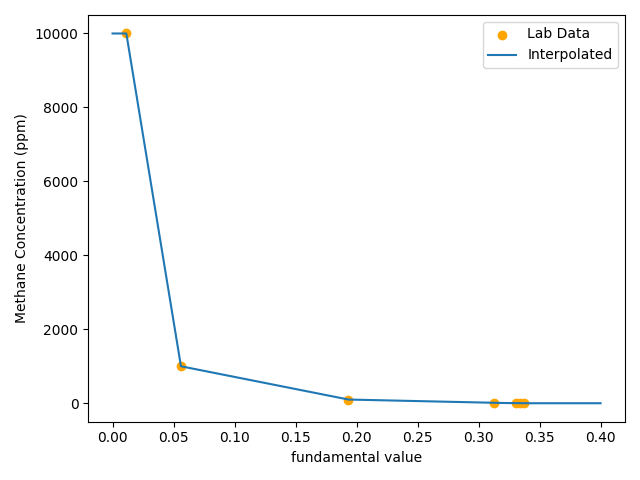
\includegraphics[width=0.6\textwidth]{figures/nopp_fundamental_calib_inverted.png}
    \caption{Fitted calibration curve for measurements of methane observed by Pythia.}
    \label{fig:nopp_curve}
\end{figure}

Compensation of Pythia's time response was also performed on post-calibrated data using the methodology described in \cite{miloshevich2004development} with a smoothing window of 5 minutes, and subsampling at a quarter of the time delay window. This methodology is sensitive to noise in the signal, which motivates the extreme sub-sampling that is performed. Fig.~\ref{fig:fund_corrected} shows the effect of smoothing, time-correction, and conversion on the direct signal recorded by Pythia before normalization. 

\begin{figure}[h!]
    \centering
    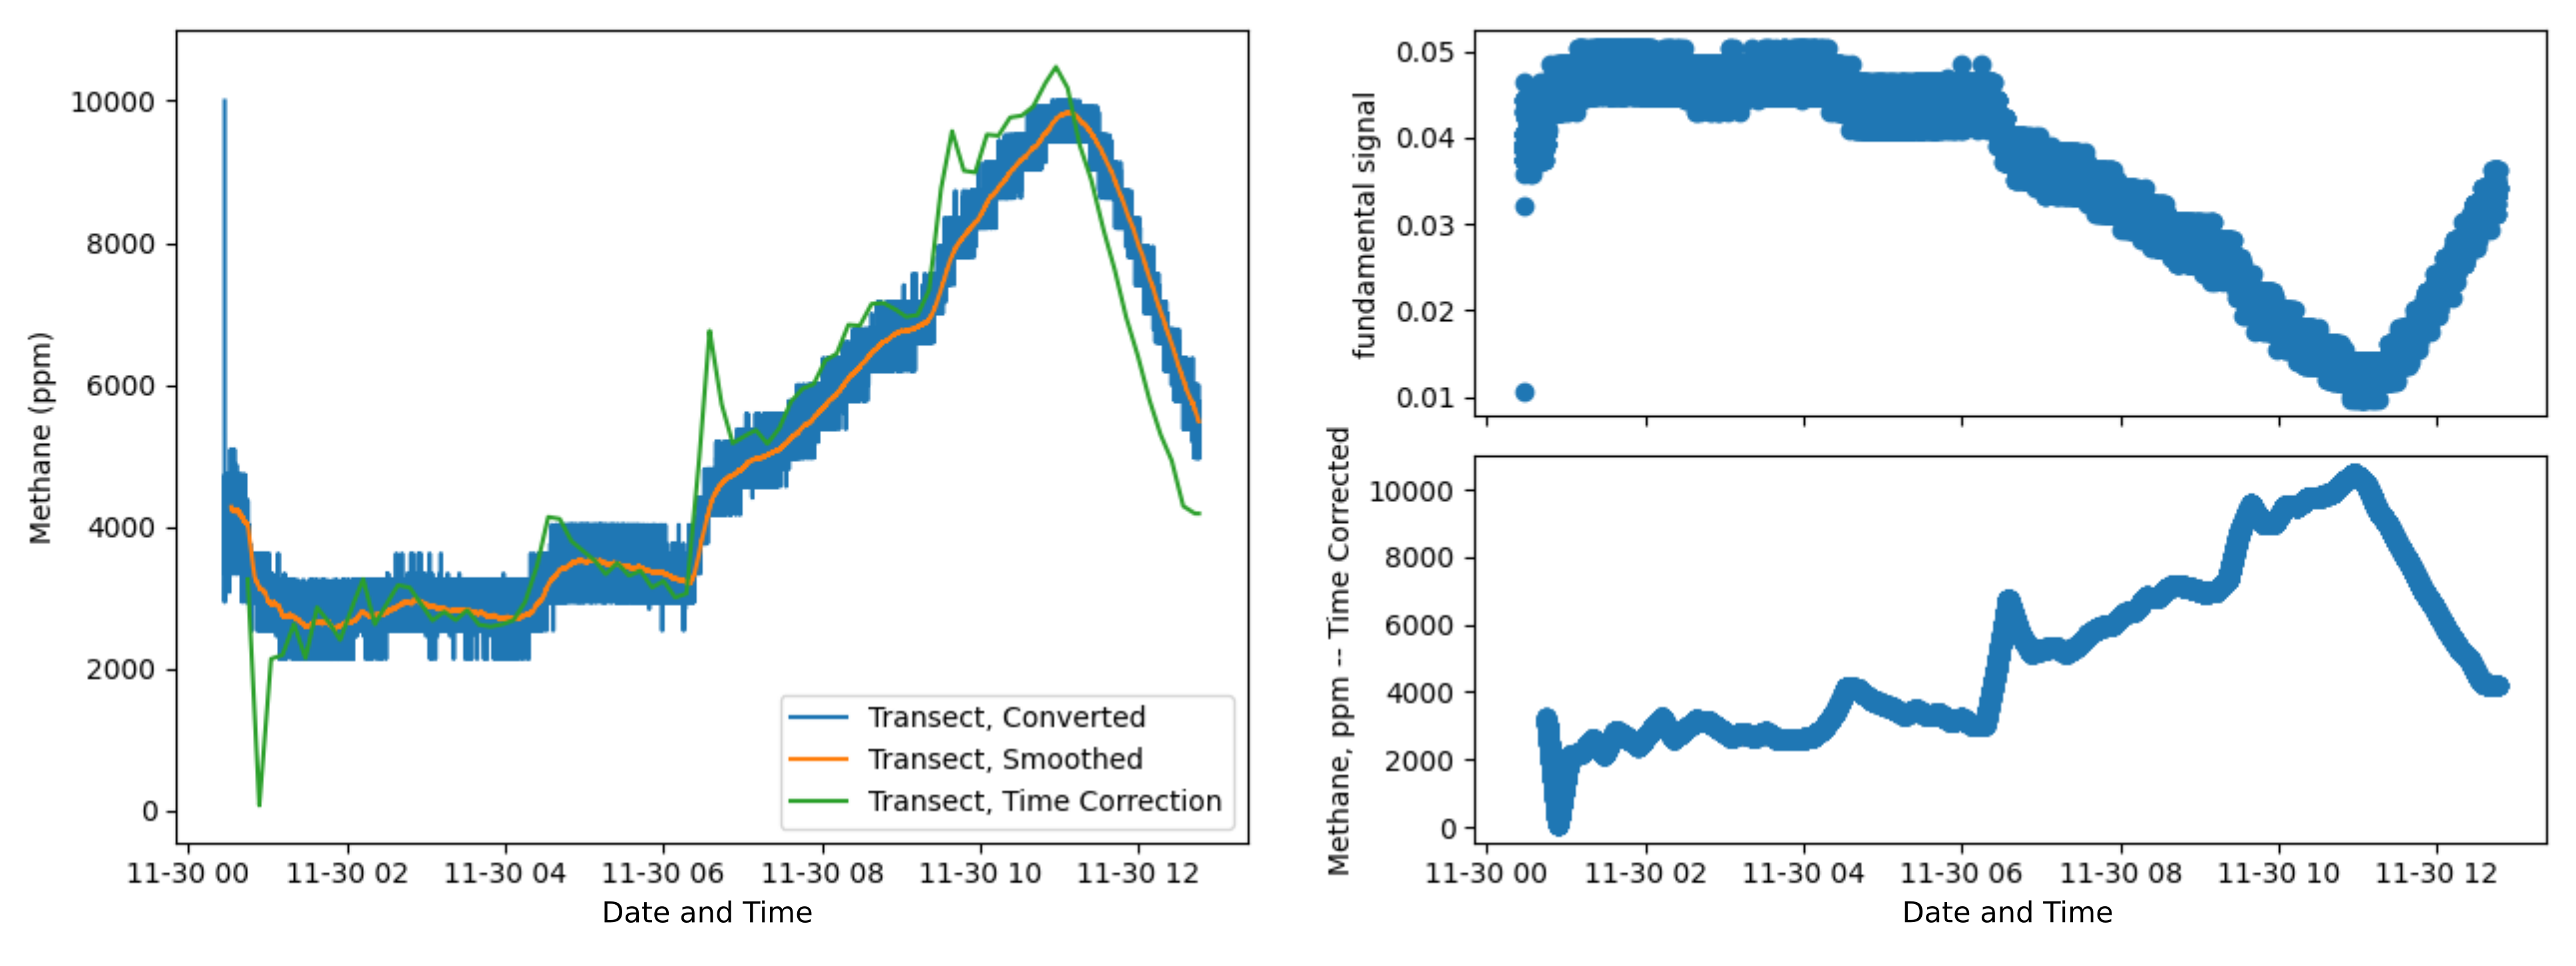
\includegraphics[width=1\textwidth]{figures/pythia_calibration.png}
    \caption[Pythia calibrated field data]{Calibration curve, smoothing, and time correction applied to Pythia observations during the transect, before reported normalization in the manuscript.}
    \label{fig:fund_corrected}
\end{figure}


\section{Depth-Correction}
\label{app:perception:depth}
Temperature, salinity, and oxygen are expected to be weakly stratified in the deep ocean. To remove these effects from data collected by AUV Sentry and the rosette, we fit a line to the average observations collected within binned 20 m intervals of observed depth for each platform separately. Separately computing the correction for each instrument additionally controls for small discrepancies in calibration between the platforms. Fig.~\ref{fig:linear_fits} compares these lines with the observations collected.

\begin{figure}[h!]
    \centering
    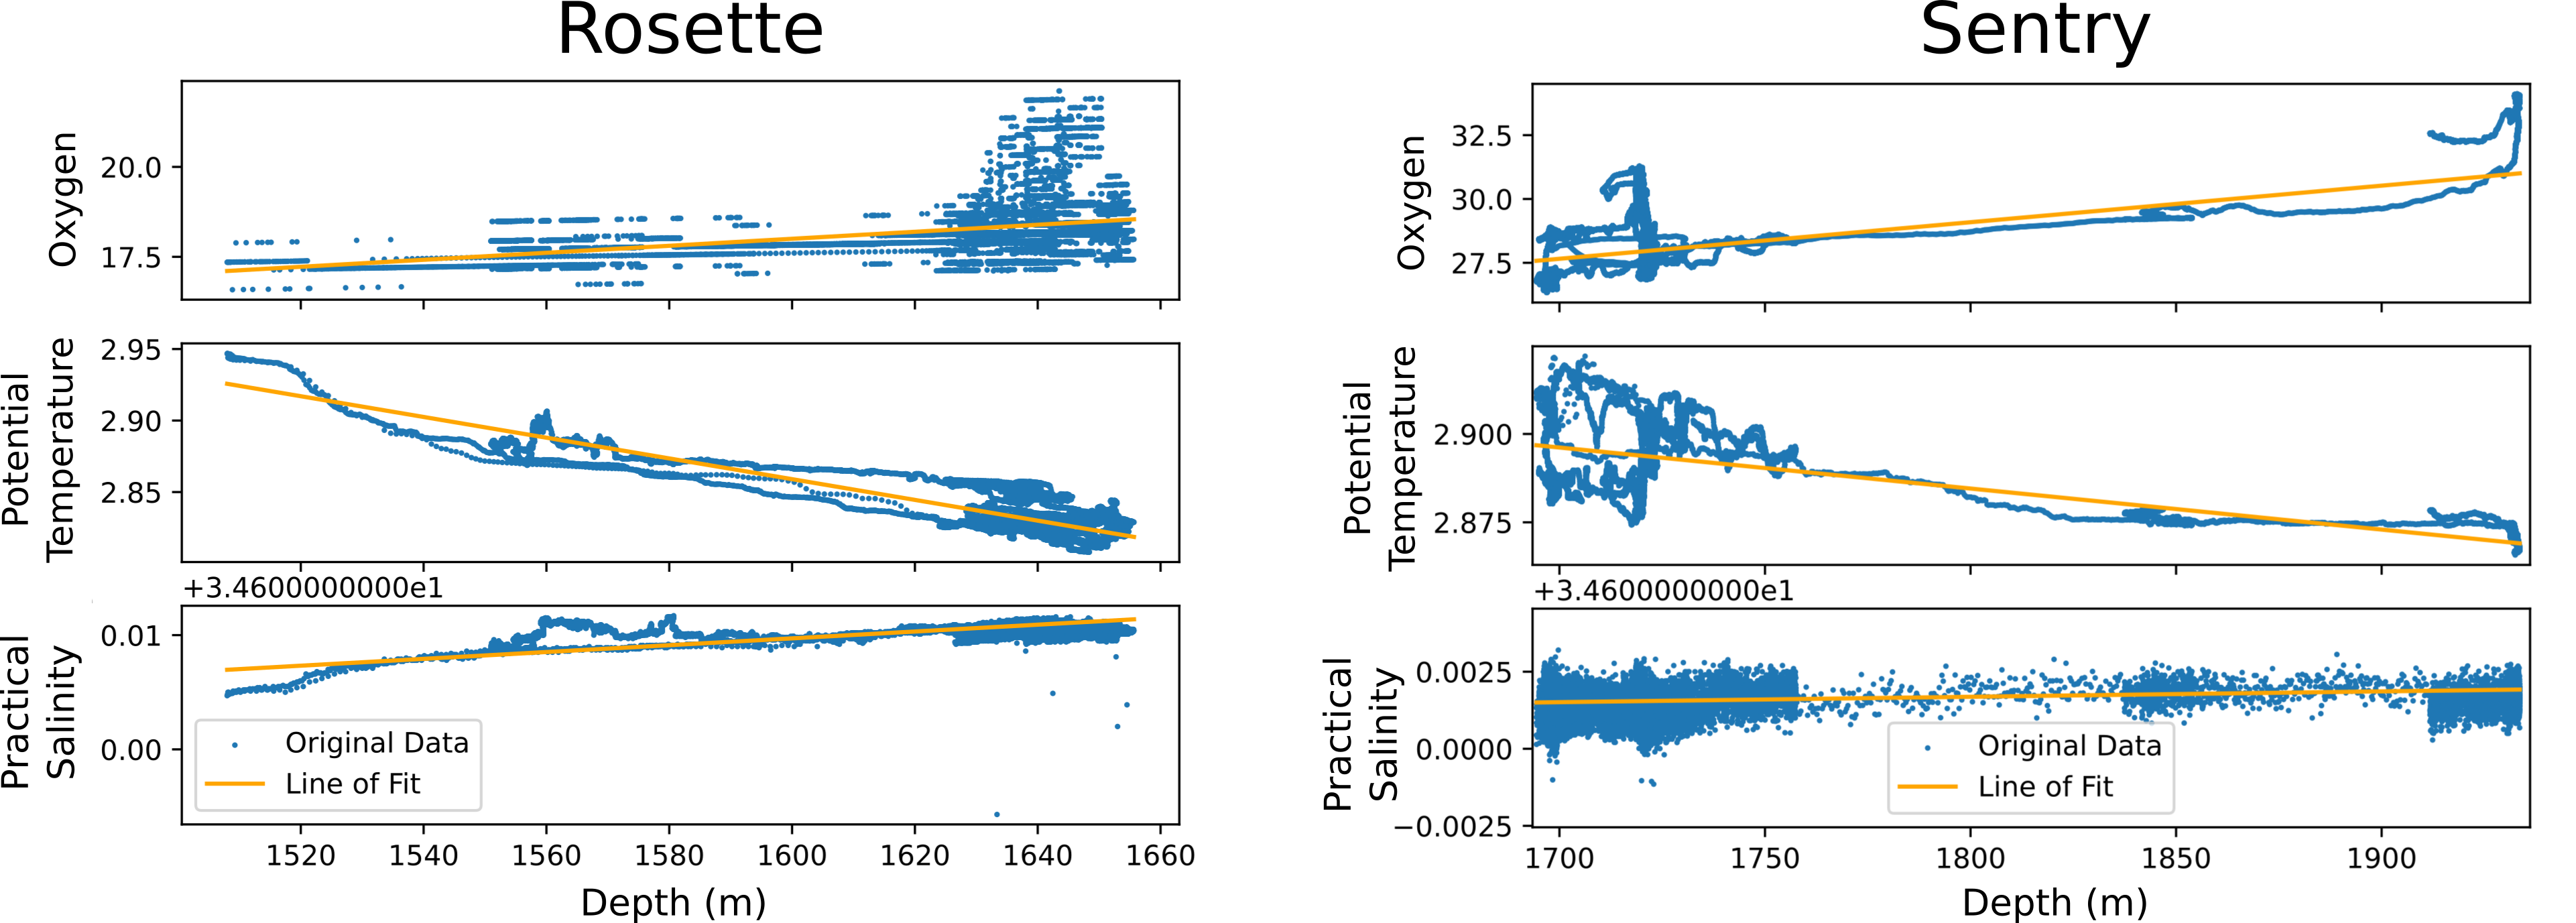
\includegraphics[width=1\columnwidth]{figures/depth_correction_plots.png}
    \caption[Functions used for depth normalization]{Linear functions are fit to data collected for oxygen, temperature, and salinity instruments on each platform separately. A residual value is then computed for each observation.}
    \label{fig:linear_fits}
\end{figure}

\section{Description of Plume Model for Transect Design}
\label{app:perception:model}
We adapted an idealized buoyant bent-plume model proposed by \cite{tohidi2016highly} for atmospheric bent plumes in a weakly stratified fluid in order to inform at what heights to deploy AUV Sentry and the rosette during the transect. We rewrite the system of equations provided in \cite{tohidi2016highly} as follows:

\begin{align}
    E &= \alpha\left|\frac{M}{Q} - u\cos(\theta)\right| + \beta\left|u\sin(\theta)\right| \\
    \frac{dQ}{ds} &= QE\sqrt{\frac{2(1 + \lambda^2)}{M\lambda}} \\
    \frac{dM}{ds} &= u\cos(\theta)\frac{dQ}{ds} + \frac{FQ}{M}\sin(\theta)\\
    \frac{d\theta}{ds} &= \left(\frac{FQ}{M}\cos(\theta) - u\sin(\theta)\frac{dQ}{ds}\right)\frac{1}{M}
\end{align}
\begin{align}
    \frac{dF}{ds} &= -QN^2\sin(\theta)\\
    \frac{dX}{ds} &= \cos(\theta)\\
    \frac{dZ}{ds} &= \sin(\theta)
\end{align}

\noindent where $E$ is a mixing entrainment coefficient which considers both vertical and horizontal mixing and is weighted by parameters $\alpha$ and $\beta$, $u$ is the crossflow velocity which can be a function of depth and time, $\lambda$ is a parameter which modifies the ellipse which describes the plume envelope, $Q$ is specific volume flux, $M$ is specific momentum flux, $F$ is specific buoyancy flux, $\theta$ is plume centerline trajectory angle, $s$ is the plume centerline trajectory, $X$ is distance along a coordinate axis aligned with the plume centerline, $Z$ is height with respect to plume source along a vertical axis, and $N^2$ is the Brunt-V\"ais\"al\"a frequency, computed with respect to the density gradient at the reference depths of the source and plume height.

The system of equations essentially yields a ``snapshot'' of a plume envelope at some moment in time. For time-varying crossflows, multiple snapshots can be computed for different moments in time (different crossflow orientations and magnitudes) and chained together in a common coordinate reference system in order to track a plume trajectory. For the purposes of determining which heights to deploy AUV Sentry and the rosette for the transect, we compute a prototypical envelope and use the estimated bent nonbuoyant plume height to set the transect depths/altitudes.

The initial conditions for solving this system of ordinary differential equations are set via estimates of vent characteristics including exit velocity, temperature, salinity, and area. Specifically:

\begin{align}
    Q_o &= \lambda V_v \frac{A_v}{\pi} \\
    M_o &= Q_o V_v \\
    F_o &= -g10^{-4}(T_v - T_z)Q_o \\
    \theta_o &= \frac{\pi}{2}
\end{align}

\noindent where $V_v$ is exit velocity at the vent orifice, $A_v$ is the vent orifice area, $T_v$ is the temperature at the orifice area, and $T_z$ is the expected temperature of ambient seawater at the estimated vent depth. Note that initial buoyancy flux is primarily driven by temperature changes, as we anticipate this to be the major driver of density gradients at our measurement scale. Expected salinity gradients could be similarly considered.

Estimated vent characteristics and crossflow were selected based on empirical observations of the deep sea vents located along the northern Guaymas Basin ridge and observations of current magnitude collected by a current tiltmeter deployed by ROV Jason during several days of the research cruise. Table~\ref{tab:params} lists the settings for planning the transect selected for these characteristics. Background salinity and temperature profiles were computed according to standard Pacific Ocean temperature and salinity functions as described in \cite{speer1989model}; additionally the equation of state for computing density profile from salinity and temperature measurements was used also as defined in \cite{speer1989model}. The prototypical plume is computed with a source located at 1850 m depth.

\begin{table}[h!]
    \centering
    \begin{tabular}{c|c|l}
        Parameter & Assignment & Description \\
        \hline
        $\lambda$ & 1.0 & Ratio of elliptical axes of the plume envelope \\
        $V_v$ & \SI{0.58}{\meter\per\second} & Exit velocity of fluids at vent orifice \\
        $A_v$ & \SI{0.82}{\meter\squared} & Area of vent orifice \\
        $T_v$ & \SI{340}{\celsius} & Temperature of fluids at vent orifice \\
        $\alpha$ & 0.15 & Longitudinal shear-driven mixing coefficient \\
        $\beta$ & 0.19 & Transverse shear-driven mixing coefficient \\
        $u$ & \SI{0.1}{\meter\per\second} & Magnitude of crossflow \\
    \end{tabular}
    \caption{Parameter, vent characteristics, and ambient crossflow setting used for transect design.}
    \label{tab:params}
\end{table}

The prototypical plume envelope computed in this manner estimates a nonbuoyant plume depth between 1570-1750 m (Fig.~\ref{fig:plume_envelopes}). AUV Sentry is altitude limited in order to keep a fix on the ocean floor for navigation; it is set to its maximum altitude of \SI{120}{\meter} in order to intersect with the bottom of the estimated nonbuoyant layer; this corresponds to a depth of approximately 1700 m throughout the basin. The rosette can be arbitrarily fixed to a height, but so as not to interfere with AUV Sentry operations and to sample a different point in the estimated nonbuoyant layer, a depth of 1650-1600 m was targeted.

\begin{figure}[h!]
    \centering
    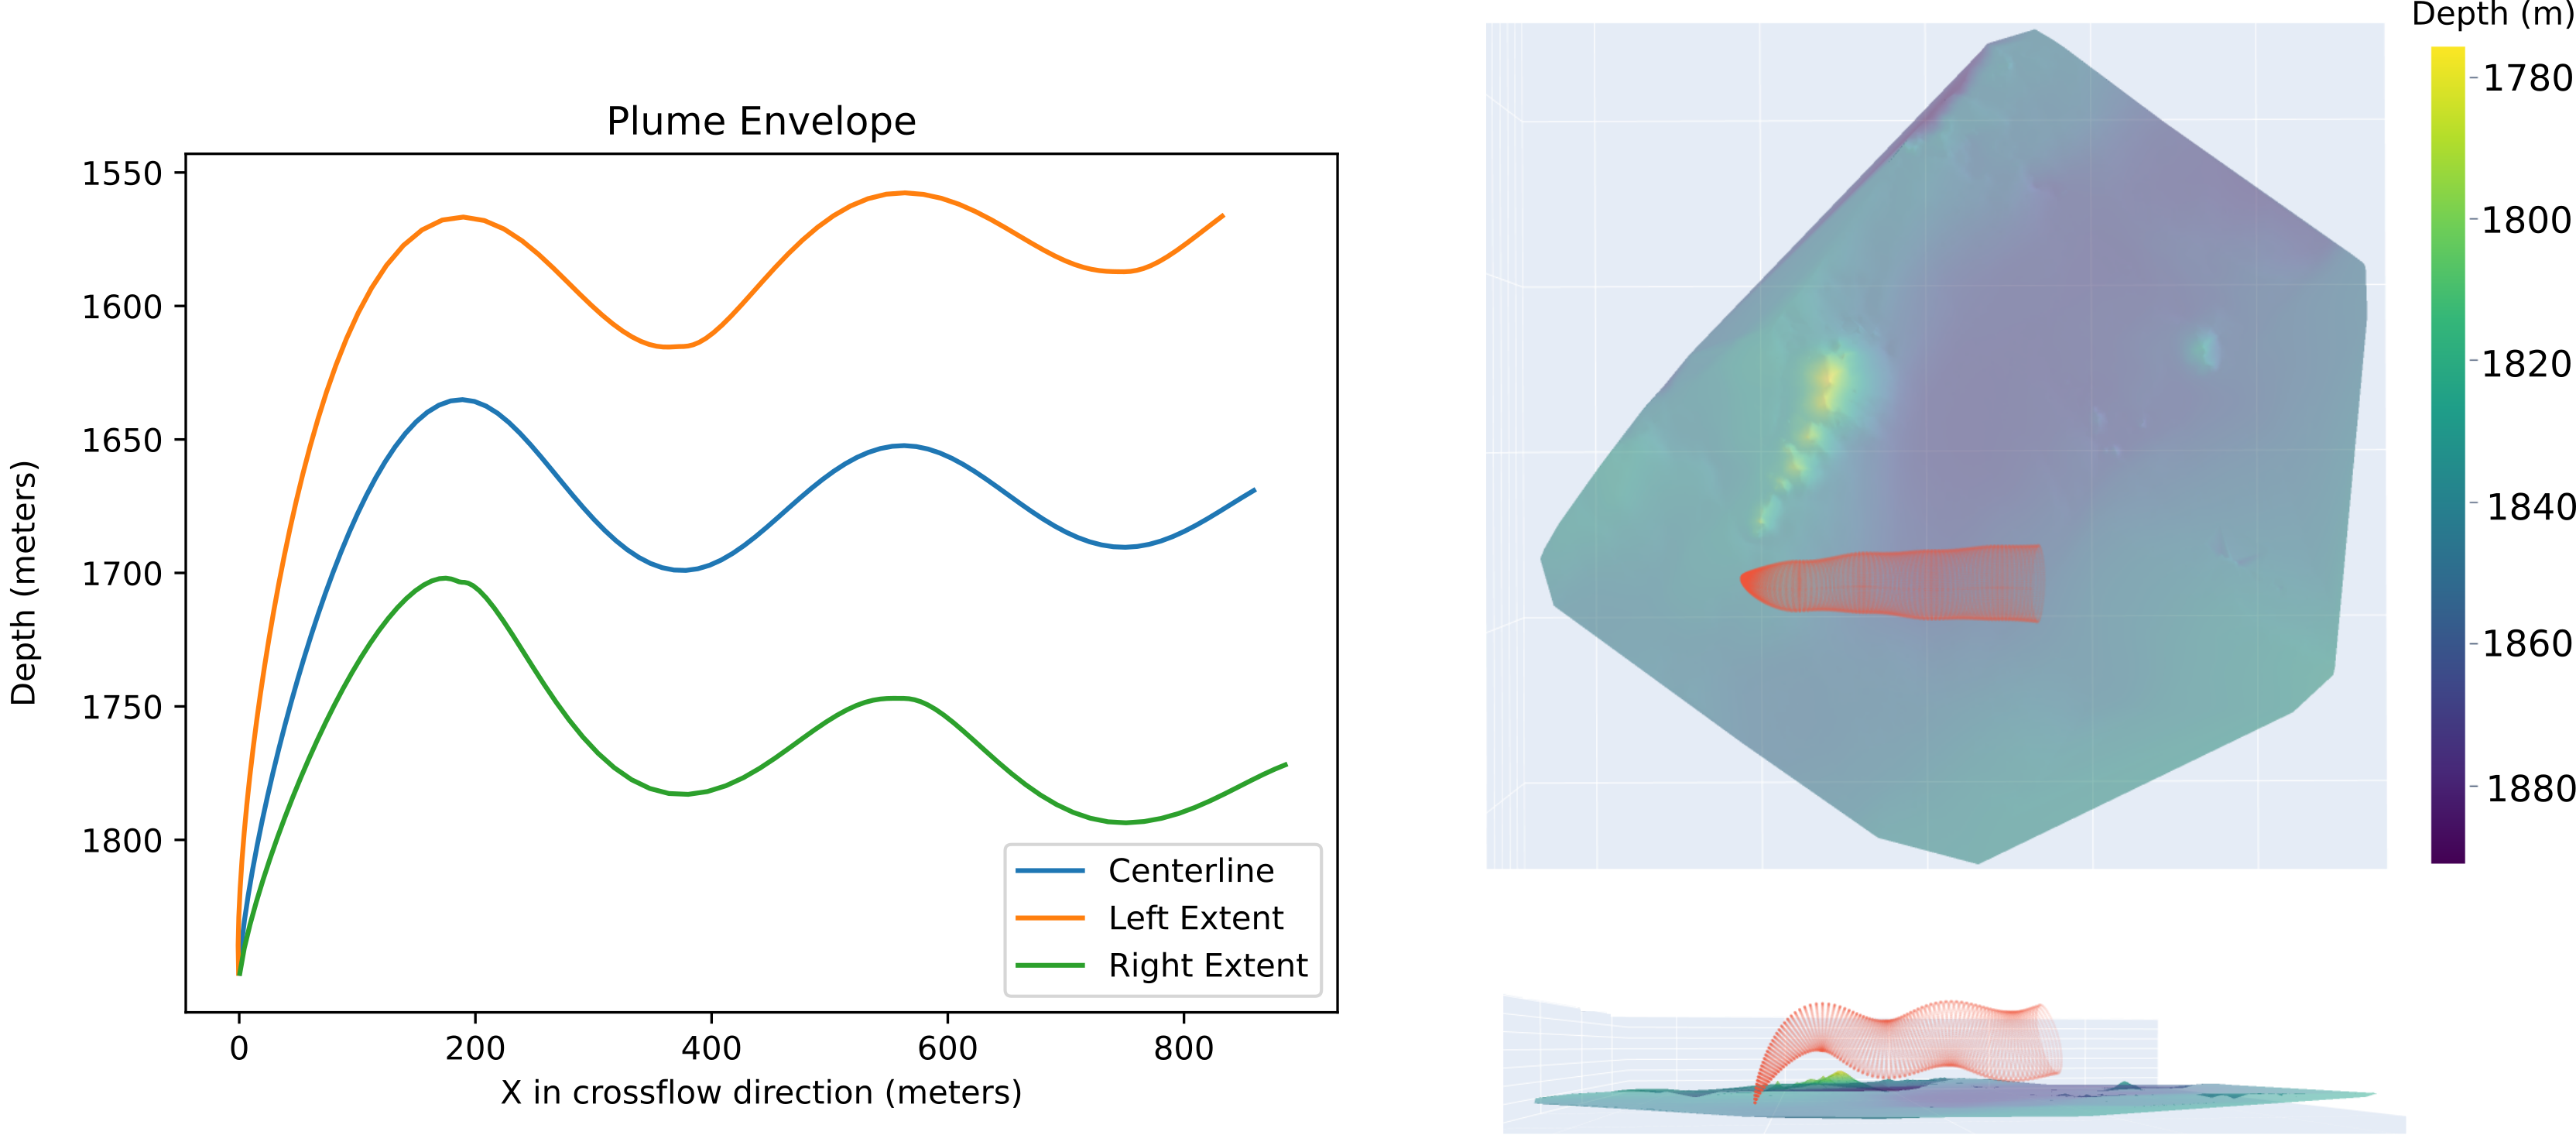
\includegraphics[width=1\columnwidth]{figures/plume_envelopes.png}
    \caption[Plume model for transect design]{A prototypical plume estimate according to the modified buoyant plume model in crossflow. The same envelope is plotted with respect to absolute depth (with a source located at 1850 m) on the left, and illustratively in the context of the hydrothermal ridge on the right.}
    \label{fig:plume_envelopes}
\end{figure}

%%%%%%
% Appendix B
%%%%%%
\chapter{\PHORTEX Algorithm Performance}
\label{app:phortex}

\section{Convergence Characteristics of Trajectory Optimizer}
The trajectory optimization scheme presented in \cref{sec:to} uses a gradient-based optimizer with trust-bounded constraints in order to set the parameters of a set of lawnmower trajectories. In general, this is a difficult optimization problem, as analytical gradients that map the defining parameters of a lawnmower trajectory (orientation, size, and location) are not available, and must be numerically approximated. Moreover, by defining trust constraints, jumping between minima could be made more difficult, as the approximated gradients may lead through unsafe (un-trusted) space. In practice, this meant that initializing each lawnmower in a chain to be near a ``good trajectory'' was important. In the case of charting hydrothermal plumes, a ``good'' trajectory would be one approximately aligned with the estimated crossflow. As \PHUMES provides complete access to this information, it is generally easy to seed the trajectories to be near a performant minima. This leads to relatively fast convergence of the optimizer for each element in the chain. In \cref{fig:phortex_chain} there is an example a snapshot along the path to convergence for each link in a chain visualized, and the convergence plot. As is evidenced in the plot, a long travel time between chains is accumulated; this is likely because ``flipping'' a trajectory to shorten this distance would be a prohibitively difficult step in the nonlinear, constrained space that the optimizer operates.

\begin{figure}[h!]
    \centering
    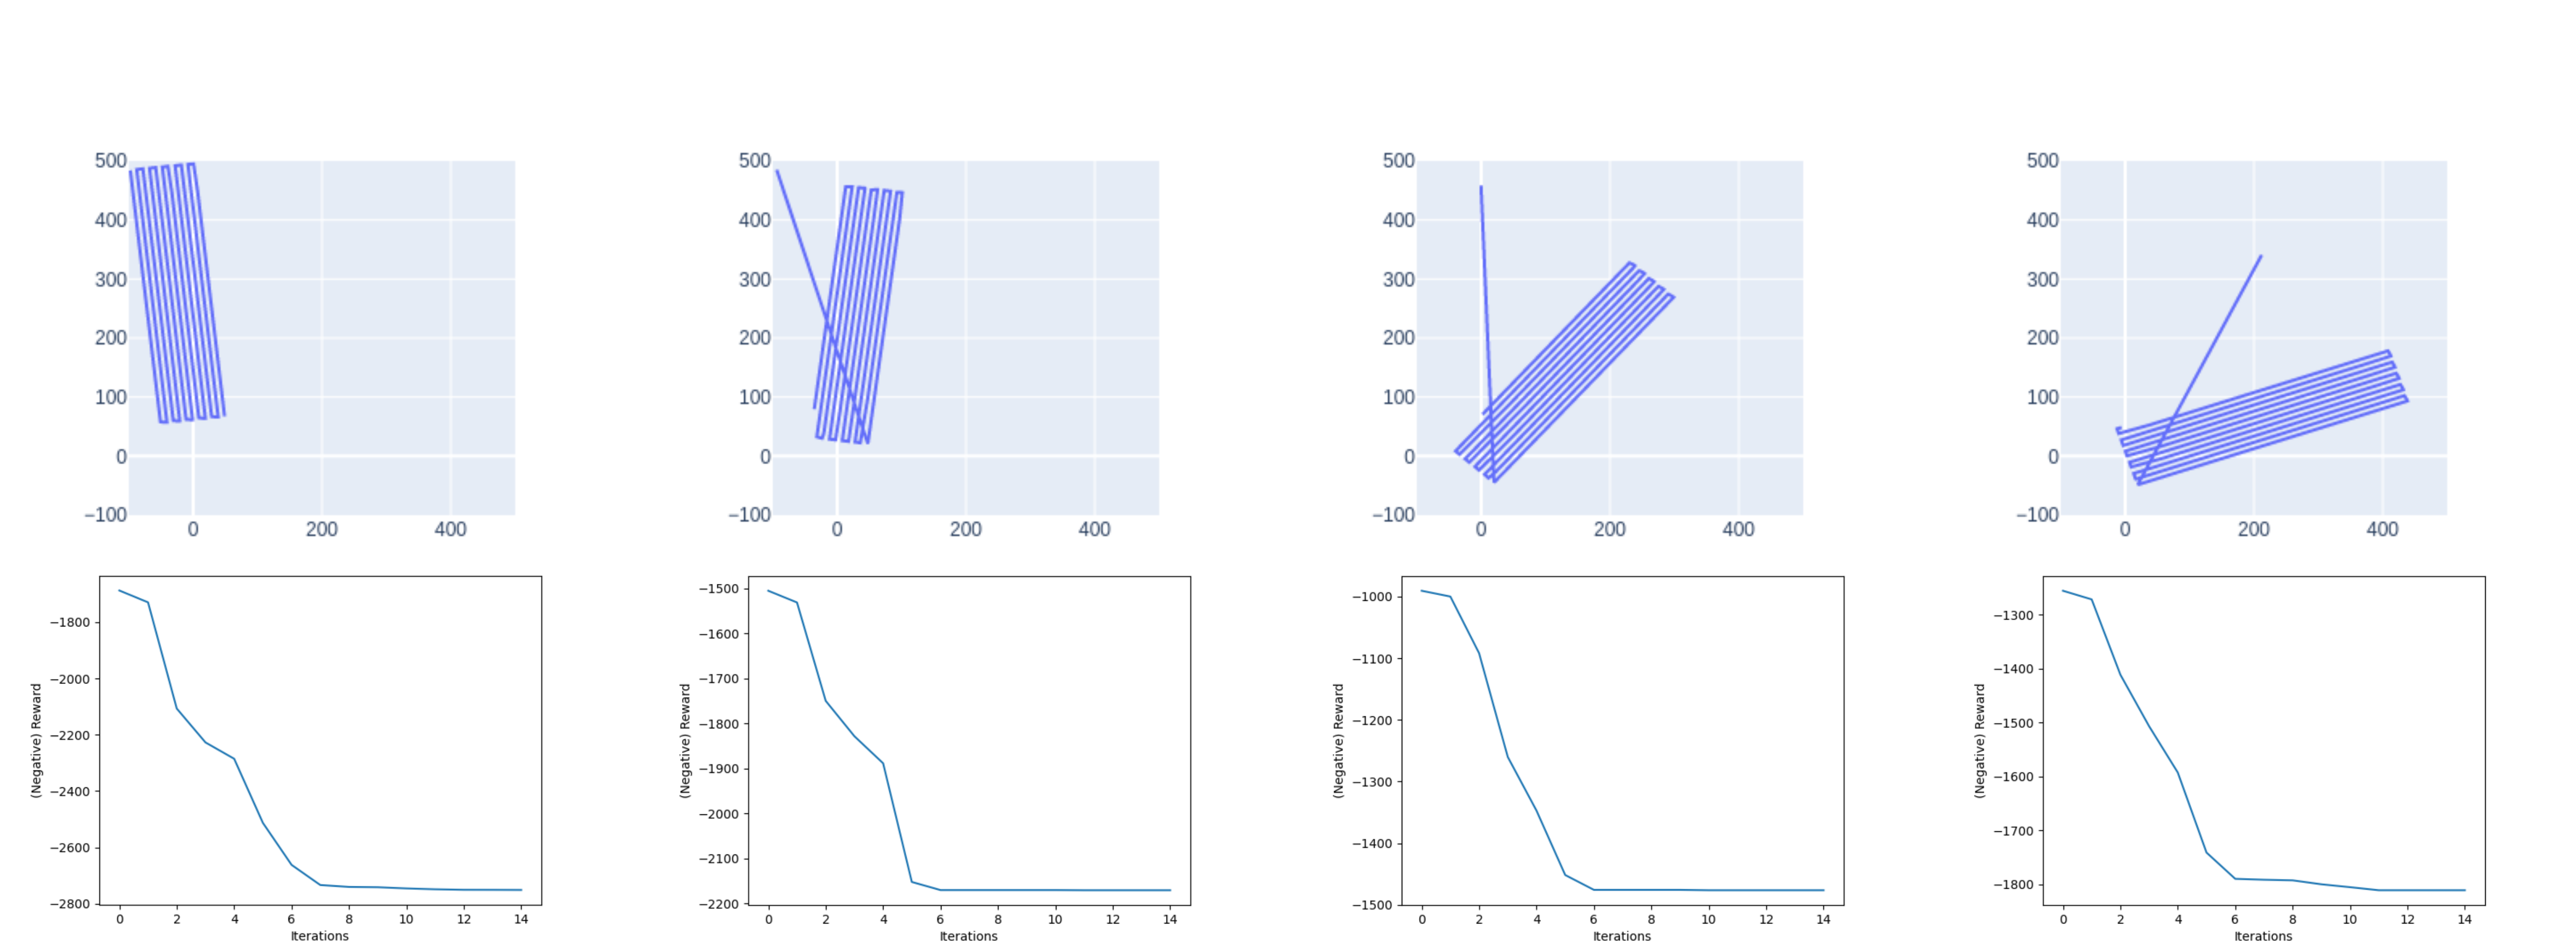
\includegraphics[width=1\columnwidth]{figures/phortex_iterations.png}
    \caption[\PHORTEX optimization performance]{Example snapshots of each link in a \PHORTEX trajectory from a \cref{chap:phortex} simulation trial, and their corresponding convergence plots. While trajectories show good agreement with the current function and size of a plume expression as modeled by \PHUMES, a long travel time between chains is accumulated; this is likely because ``flipping'' a trajectory to shorten this distance would be a prohibitively difficult step in the nonlinear, constrained space that the optimizer operates.}
    \label{fig:phortex_chain}
\end{figure}

\section{Chaining Characteristics of \PHUMES}
For computational reasons, it is typically not possible to run the chains for thousands of samples while in the field, and the chains must be arbitrarily cut short in order to generate a plan. For this reason, it is interesting to look at the chaining properties. For a simulation trial, as described in \cref{chap:phortex}, we show the chains and probability densities for each of vent area, vent fluid velocity, and entrainment coefficients in \cref{fig:phumes_sim_chain}. As evidenced by the multimodal area plot, we observe that the relationship between the parameters is complicated; in general, an inverse problem like the one we have posed for \PHUMES is a challenge to infer. What is promising however is that probability densities are being concentrated in areas that make sense (as observed by a mode at 0.8 for area), and that the \emph{combinations} of learned parameters are sensible --- a large area should be coupled with a slow or medium velocity; a high velocity should be paired with a small area --- based on the relationships between parameters and how they manifest in the ultimate shape of the plumes in the 3D Cartesian space.

\begin{figure}[h!]
    \centering
    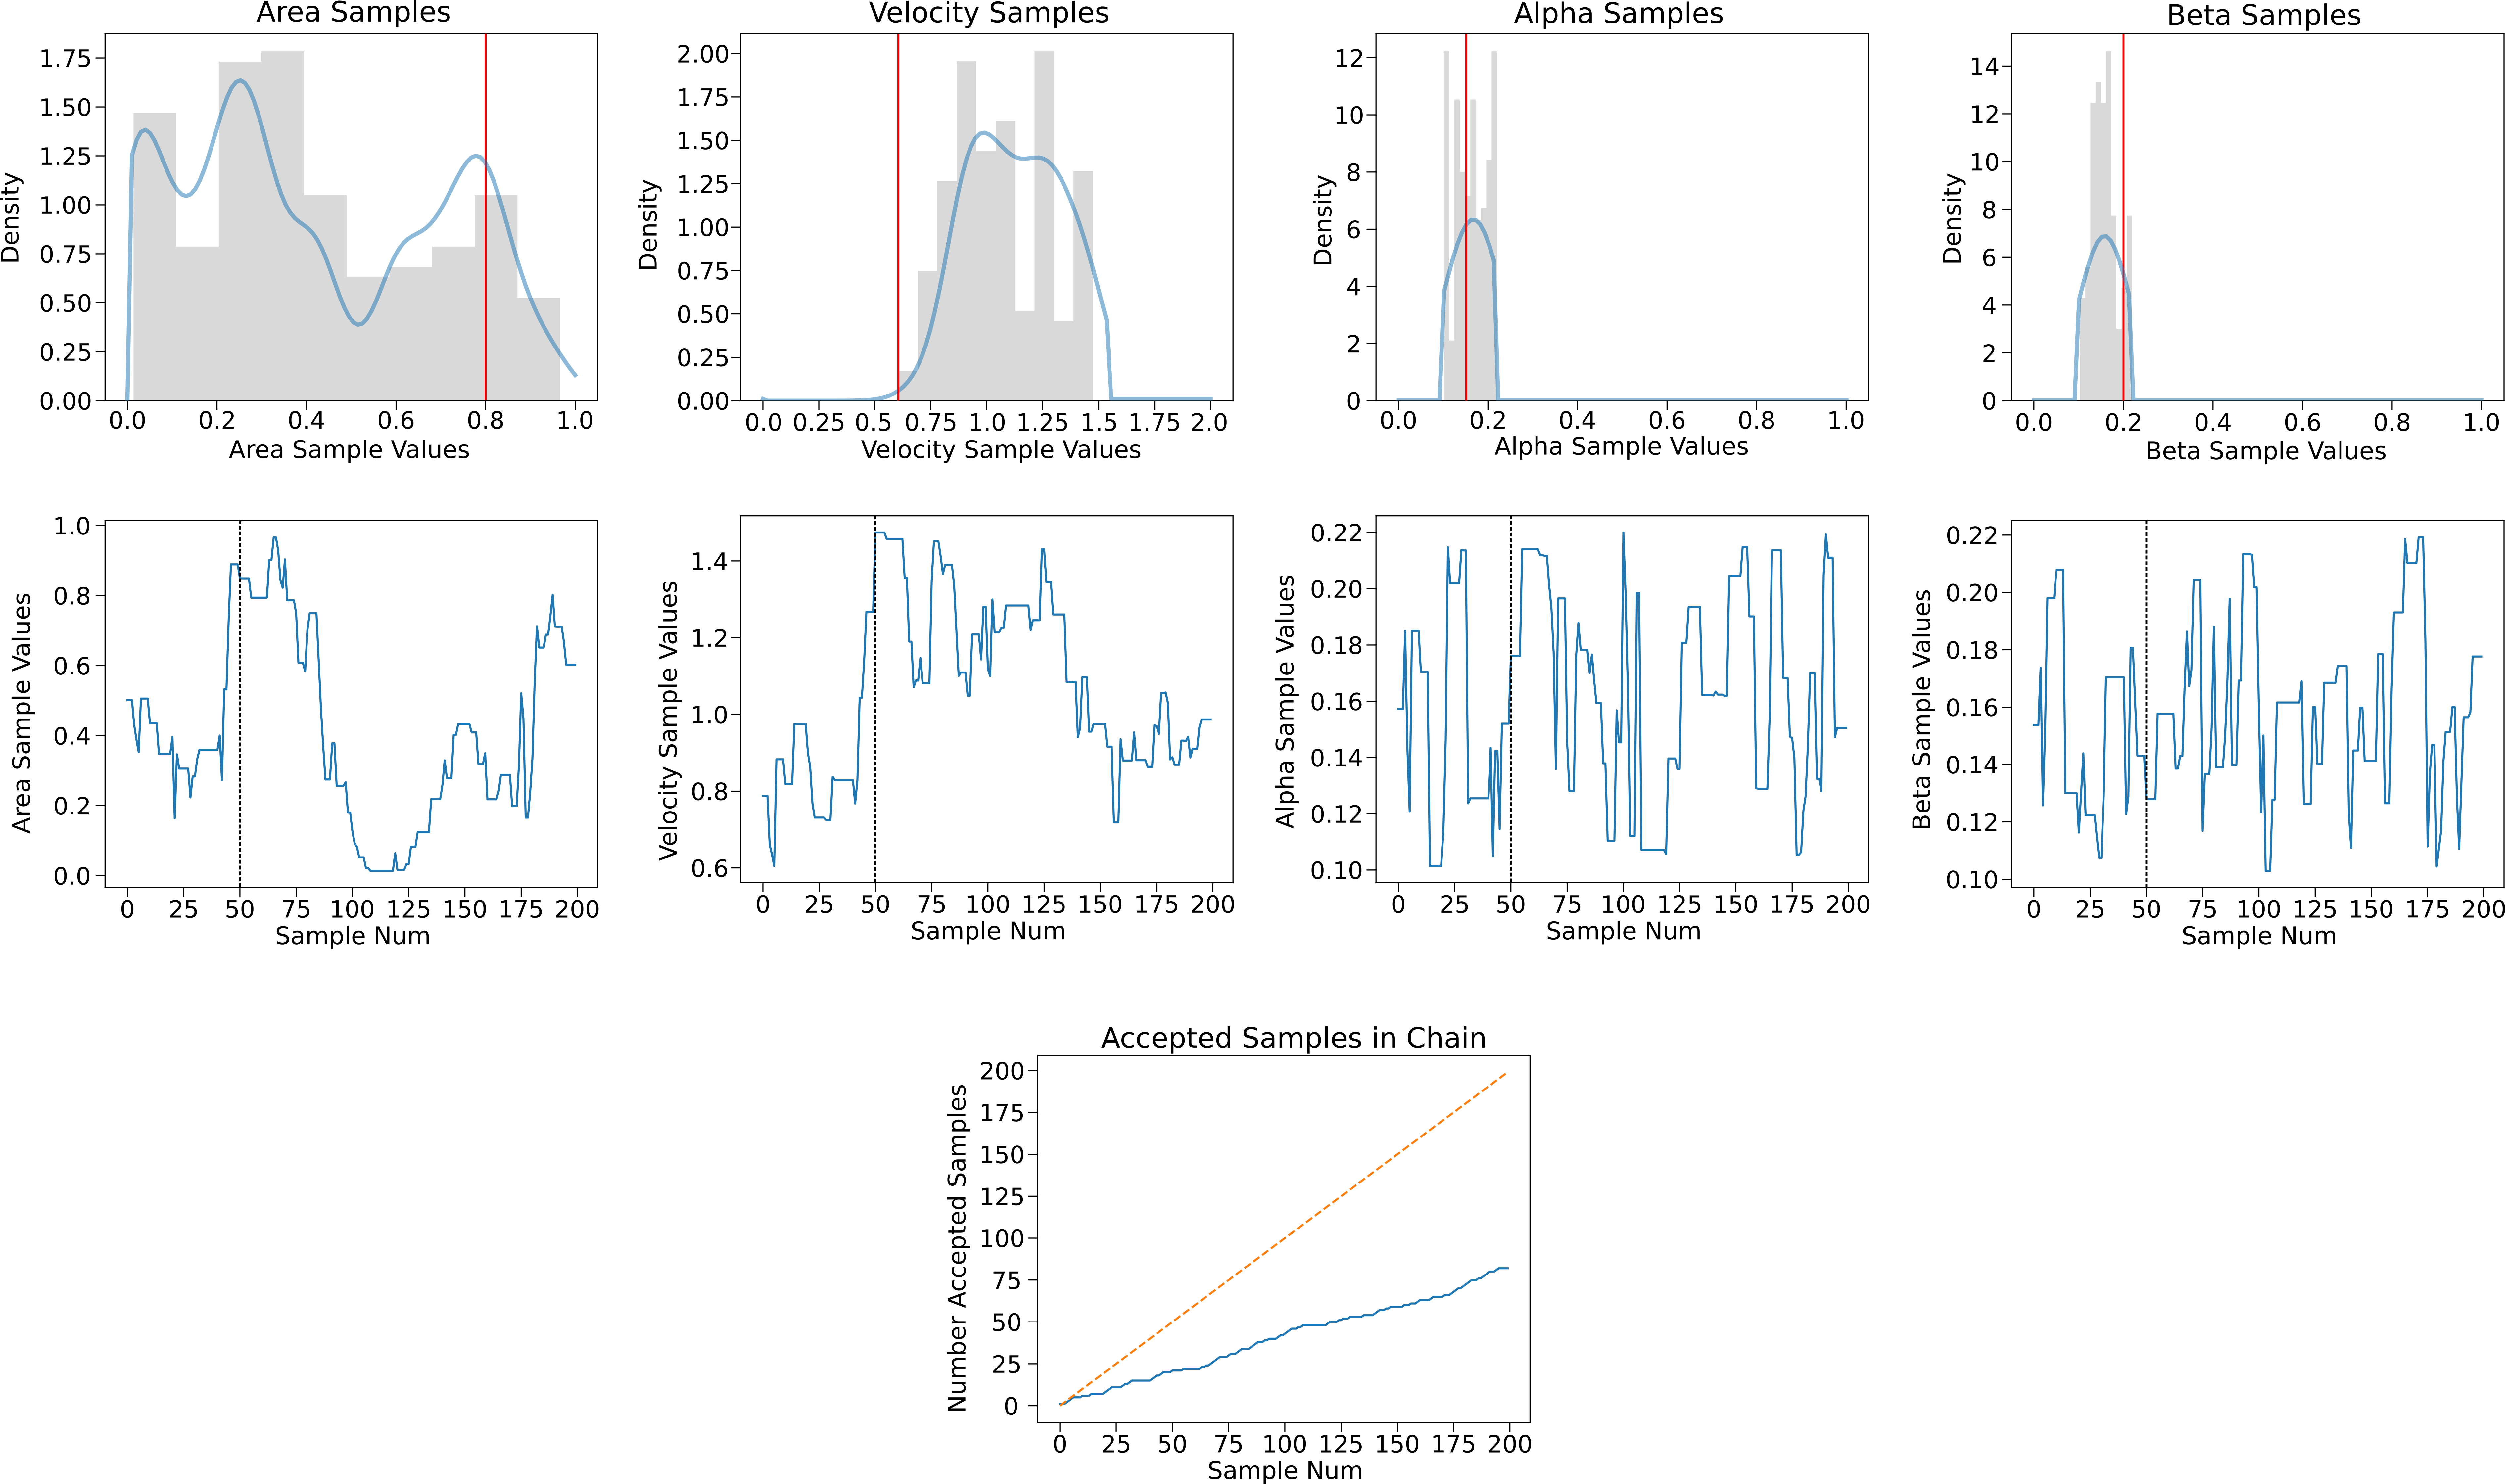
\includegraphics[width=1\columnwidth]{figures/phumes_trial_chain.png}
    \caption[\PHUMES simulation chain]{An example chain from a simulation trial as described in \cref{chap:phortex}. The last 150 samples in each chain is used to compute the distributions in blue; all samples are shown in gray in the top plots. Red lines in the top plots indicate the generating environment value for the simulation. The chain efficiency is approximately 37.5\%.}
    \label{fig:phumes_sim_chain}
\end{figure}

We can also look at how convergence may change for longer chains. In an exemplar trial (\cref{fig:phumes_long_chain}), a chain is run for 650 samples, and the last 500 samples are used to compute densities. The acceptance rate stays approximately the same, at about 34\%. However, the distributions have generally improved with respect to placing more density at the parameters that defined the true underlying environment. As evidenced in the area and velocity sampling plots, there is still some exploration of the state space being performed by the chains; this suggests that true convergence of these chains may either take a long time, or the information content of the data that is available to explore the state space leads to ambiguous ``wells'' which the chains would ``bounce'' between for long durations. This suggests that other Monte Carlo techniques, such as Hamiltonian Monte Carlo~\autocite{duane1987hybrid}, may be of interest in adaptation of this work, to accelerate chain exploration.

\begin{figure}[h!]
    \centering
    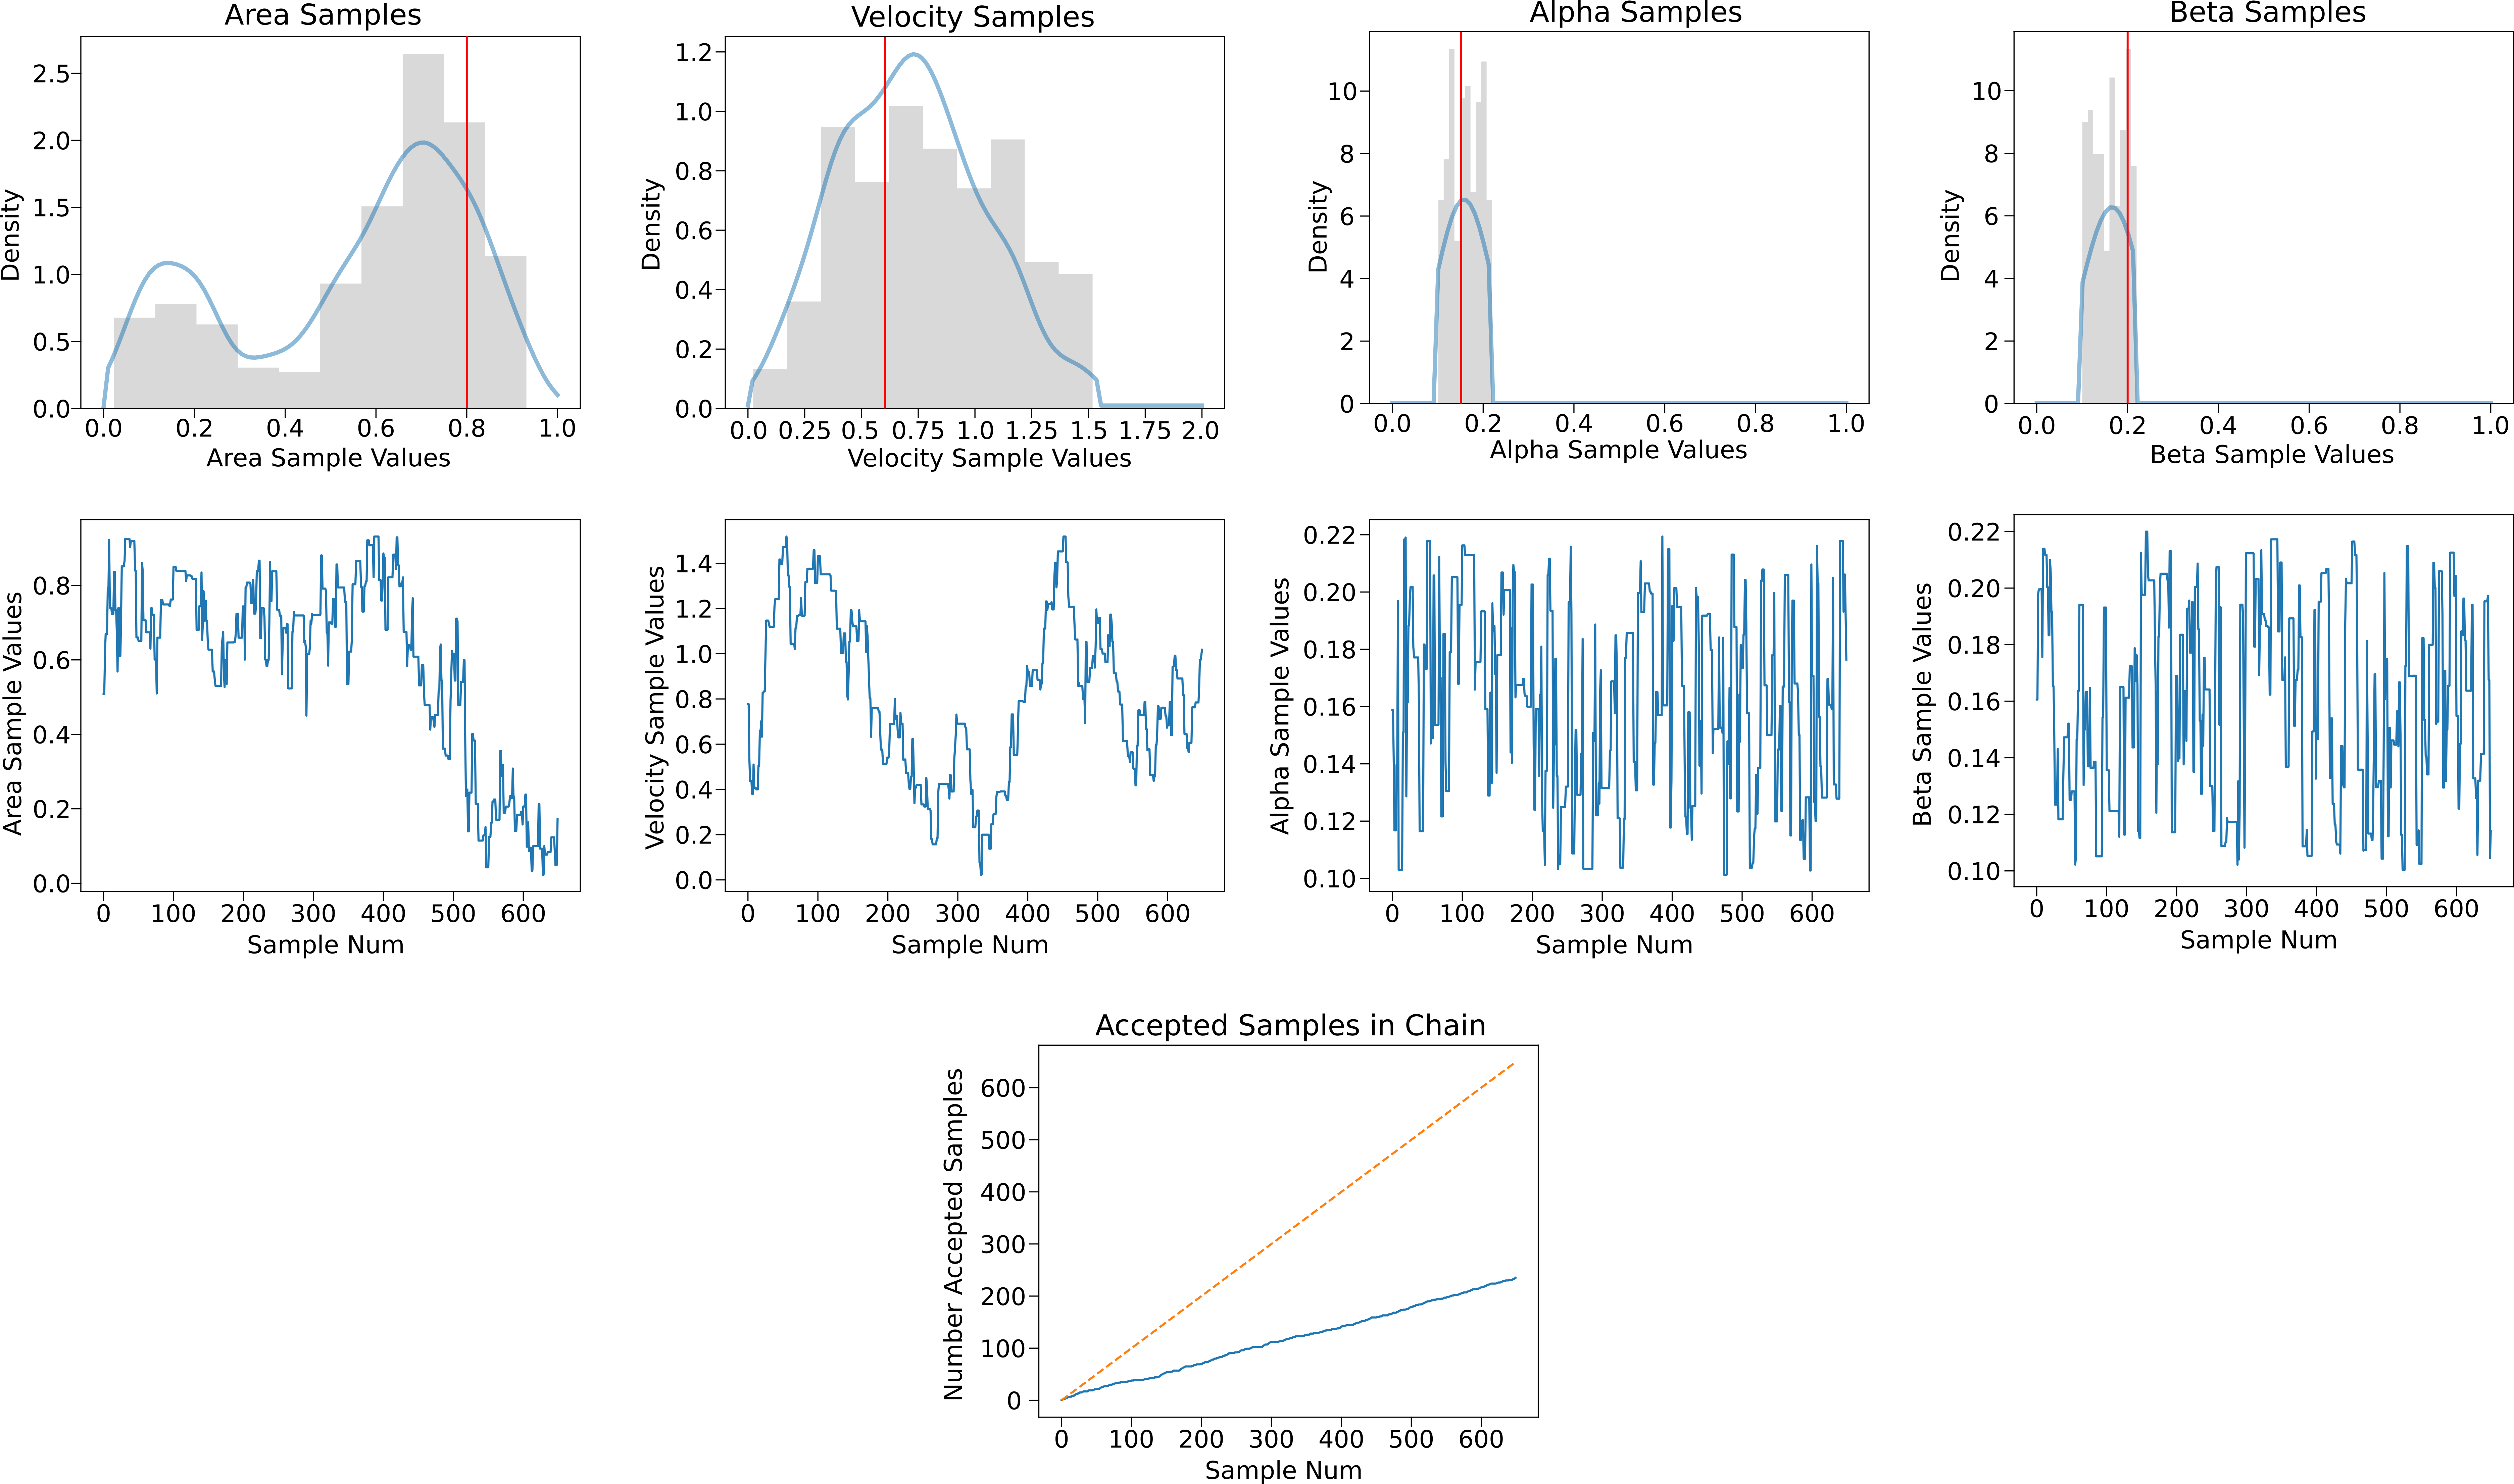
\includegraphics[width=1\columnwidth]{figures/phumes_long_chain.png}
    \caption[\PHUMES long chain]{An example chain from a simulation trial as described in \cref{chap:phortex}, but run for 650 samples; the last 500 are used to compute the distributions in blue with all samples shown in gray in the top plots. Red lines in the top plots indicate the generating environment value for the simulation. The chain efficiency is approximately 34\%.}
    \label{fig:phumes_long_chain}
\end{figure}

\section{Code Availability}
\td{Might be nice to link to the code here and have some brief documentation on how to use it.}

%% This defines the bibliography file (main.bib) and the bibliography style.
%% If you want to create a bibliography file by hand, change the contents of
%% this file to a `thebibliography' environment.  For more information 
%% see section 4.3 of the LaTeX manual.
\begin{singlespace}
    \bibliography{bibliography/biblio}
    \bibliographystyle{plain}
\end{singlespace}
    
\end{document}

